\chapter{Конвергенция и интеграция искусственных нейронных сетей с базами знаний в ostis-системах}
\chapauthortoc{Ковалёв М.В.\\Крощенко А.А.\\Головко В.А.}
\label{chapter_ann}

\vspace{-7\baselineskip}

\begin{SCn}
	\begin{scnrelfromlist}{автор}
		\scnitem{Ковалёв М.В.}
		\scnitem{Крощенко А.А.}
		\scnitem{Головко В.А.}
	\end{scnrelfromlist}

	\bigskip

	\scntext{аннотация}{В главе рассмотрен подход к интеграции и конвергенции искусственных нейронных сетей с базами знаний в интеллектуальных компьютерных системах нового поколения с помощью представления и интерпретации искусственных нейронных сетей в базе знаний. Описаны синтаксис, денотационная и операционная семантика языка представления нейросетевых методов в базах знаний. Описаны этапы построения нейросетевых методов решения задач с помощью интеллектуальной среды проектирования искусственных нейронных сетей.}

	\bigskip

	\begin{scnrelfromlist}{подраздел}
		\scnitem{\nameref{sec_chapter_ann_models}~\nameref{sec_chapter_ann_models}}
		\scnitem{\nameref{sec_chapter_ann_framework}~\nameref{sec_chapter_ann_framework}}
	\end{scnrelfromlist}

	\bigskip

	\begin{scnrelfromlist}{ключевые элементы}
		\scnitem{нейросетевой метод решения задач}
		\scnitem{язык представления нейросетевых методов решения задач}
		\scnitem{нейросетевая модель решения задач}
		\scnitem{навык решения задач с помощью искусственных нейронных сетей}
		\scnitem{действие по построению искусственных нейронных сетей}
	\end{scnrelfromlist}

	\bigskip

	\begin{scnrelfromlist}{библиографическая ссылка}
		\scnitem{\scncite{Standart2021}}
		\scnitem{\scncite{Castelvecchi2016}}
		\scnitem{\scncite{Ribeiro2016}}
		\scnitem{\scncite{Lundberg2017}}
		\scnitem{\scncite{Garcez2015}}
		\scnitem{\scncite{Besold2017}}
		\scnitem{\scncite{Golovko2019}}
		\scnitem{\scncite{Kroshchanka2022}}
		\scnitem{\scncite{Golovko2017}}
		\scnitem{\scncite{Glorot2010}}
		\scnitem{\scncite{He2015}}
		\scnitem{\scncite{Goodfellow2017}}
		\scnitem{\scncite{Haykin2006}}
		\scnitem{\scncite{Duchi2011}}
		\scnitem{\scncite{Kingma2014}}
	\end{scnrelfromlist}

\end{SCn}

\section*{Введение в Главу \ref{chapter_ann}}

Современные решатели задач интеллектуальных систем все чаще сталкиваются с необходимостью решения комплексных задач с помощью различных традиционных и интеллектуальных методов решения задач в едином информационном ресурсе (в пределе -- в единой базе знаний).

С другой стороны, интеллектуальные компьютерные системы нового поколения обладают, среди прочих, следующими способностями (см. \scncite{Standart2021}):
\begin{textitemize}
	\item способность постоянно повышать качество решения задач;
	\item способность приобретать навыки решения принципиально новых задач;
	\item способность обосновывать свои решения;
	\item способность находить и устранять ошибки в своих решения (способность к интроспекции).
\end{textitemize}

Представление различных методов решения задач в единой базе знаний обеспечивает семантическую совместимость этих методов. Решая задачу с помощью таких методов, система не взаимодействует с ними по принципу "входов-выходов"{}. Напротив, единая память позволяет отслеживать преобразование входных знаний в реальном времени с помощью любых имеющихся методов, что обеспечивает способность к интроспекции и способность объяснять решения системы.

Перспективными и активно развивающимися методами решения задач являются \textbf{\textit{искусственные нейронные сети}} (и.н.с.), что обуславливается, с одной стороны, развитием теории и.н.с, а с другой -- аппаратных возможностей машин, которые используются для их обучения.

Достоинствами и.н.с. можно назвать способность решения задач при неизвестных закономерностях, а так же способность решения задач без необходимости разработки проблемоориентированных подходов.

Большинство нейросетевых моделей работают как "черный ящик"{} (см. \scncite{Castelvecchi2016}), что является одним из основных недостатков этого метода решения задач. Большой объём обрабатываемых этими моделями данных создает необходимость мониторинга, объяснения и понимания механизмов их работы с целью вербализации оценки и оптимизации деятельности и.н.с.

Современные задачи все чаще требуют обоснования своего решения. Появилось целое направление Explainable AI, в рамках которого предпринимаются различные попытки объяснить решения и.н.с. (см. \scncite{Ribeiro2016}, \scncite{Lundberg2017}). Развиваются подходы, предлагающие интеграцию нейронных сетей с базами знаний (см. \scncite{Garcez2015}, \scncite{Besold2017}, \scncite{Golovko2019}, \scncite{Kroshchanka2022}).

Еще одним недостатком и.н.с. можно назвать эвристический характер процесса подбора архитектур моделей и параметров их обучения и высокие требования к объему знаний проектировщиков нейросетевых моделей.

Исходя из перечисленных способностей, наличие которых необходимо обеспечивать в интеллектуальных компьютерных системах нового поколения, встает проблема разработки подхода к интеграции и.н.с. в базу знаний интеллектуальной системы как в качестве метода решения задач, так и в качестве объекта автоматического проектирования новых методов. Решение этой проблемы позволит преодолеть указанные выше недостатки нейросетевого метода.

Можно выделить два основных направления интеграции и.н.с. с базами знаний:
\begin{textitemize}
	\item построение интеллектуальных систем, способных использовать нейросетевые методы наравне с другими имеющимися в системе методами для решения комплексных задач. Такие системы смогут учитывать семантику решаемых задач на более высоком уровне, что сделает решения более структурированными и прозрачными;
	\item построение интеллектуальной среды по разработке, обучению и интеграции различных и.н.с., совместимых с базами знаний через представление и.н.с. с помощью онтологических структур и их интерпретацию средствами представления знаний. Такая среда предоставит возможность интроспекции и.н.с, возможность сохранения состояний и.н.с. после обучения и реконфигурации сети, что позволит производить более глубокий анализ ее работы. Так же формальное описание знаний в рамках предметной области и.н.с. поможет уменьшить порог вхождения разработчиков в область методов решения задач с помощью и.н.с.
\end{textitemize}


\section{Модели искусственных нейронных сетей, используемых в ostis-системах}
\label{sec_chapter_ann_models}

Как уже было описано в главе \nameref{chapter_actions}, решатель задач занимается обработкой фрагментов базы знаний. На операционном уровне обработка сводится к добавлению, поиску, редактированию и удалению sc-узлов и sc-коннекторов базы знаний. На семантическом же уровне такая операция является \textit{действием, выполняемым в памяти субъекта действия}, где, в общем случае, субъектом является ostis-система, а база знаний -- ею памятью. \textit{Действие} определяется как процесс воздействия одной сущности (или некоторого множества сущностей) на другую сущность (или на некоторое множество других сущностей) в соответствии с некоторой целью.

Действия выполняются в соответствии с поставленными задачами.  \textit{Задача} -- это формальная спецификация некоторого действия, достаточная для выполнения данного действия каким-либо субъектом. В зависимости от конкретного класса задач, описываться может как внутреннее состояние самой интеллектуальной системы, так и требуемое состояние внешней среды.

Схожие задачи объединены в классы, для которых заданы обобщенные формулировки задач. Для и.н.с. выделены следующие классы задач:
\begin{textitemize}
	\item \textit{задача классификации}. Задача построения классификатора, т.е. отображения $\tilde c: X \rightarrow C$, где $ X \in \mathbb{R}^m$ -- признаковое пространство входного образа, $C = {C_1, C_2, ...C_k }$ -- конечное и обычно небольшое множество меток классов;
	\item \textit{задача регрессии}. Задача построения оценочной функции по примерам $(x_i, f(x_i))$, где $f(x)$ -- неизвестная функция. \textit{Оценочная функция} -- отображение вида $\tilde{f}: X \rightarrow \mathbb{R}$, где $X \in \mathbb{R}^m$ -- признаковое пространство входных данных;
	\item \textit{задача кластеризации}. Задача построения функции $a: X \rightarrow Y$, которая любому объекту $x \in X$ ставит в соответствие номер кластера $y \in Y$ в соответствие с определенной метрикой расстояния $\rho(x, x')$, где \textit{X} -- множество объектов, \textit{Y} -- множество номеров (имен, меток) кластеров, $x, x' \in X$;
	\item \textit{задача понижения размерности признакового пространства}. Задача построения функции $h: X \rightarrow Y$, сохраняющей заданные соотношения между точками множеств X и Y, где $X \subset \mathbb{R}^p$, $Y=h(X) \subset \mathbb{R}^q$, $q < p$;
	\item \textit{задача управления}. Задача построения модели-регулятора состояния сложного динамического объекта;
	\item \textit{задача фильтрации}. Задача построения модели, которая производит очистку исходного сигнала, содержащего некоторый шум и уменьшает влияние случайных ошибок в сигнале;
	\item \textit{задача детекции}. Является частным случаем задачи классификации и задачи регрессии. Задача построения модели, осуществляющей обнаружение объектов определенных типов на фото- и видеоизображениях;
	\item \textit{задача с ассоциативной памятью}. Задача построения модели, позволяющей выполнить реконструкцию исходного образа на основании сохраненных ранее образов.
\end{textitemize}

Для классов задач формулируются классы методов их решения. \textit{Метод решения задач} определяется как программа решения задач соответствующего класса, которая может быть как процедурной, так и декларативной. В свою очередь, \textit{класс методов решения задач} определяется как множество всевозможных методов решения задач, имеющих общий язык представления этих методов. Язык представления методов позволяет описывать синтаксическую, денотационную и операционную семантику этого метода.

Предлагается рассматривать и.н.с. как класс методов решения задач со своим языком представления. Таким образом, искусственная нейронная сеть - это \textbf{\textit{нейросетевой метод решения задач}}. В соответствии с технологией OSTIS, спецификация класса методов решения задач сводится к спецификации соответствующего языка представления методов, т.е. к описанию его синтаксической, денотационной и операционной семантики.

Для достижения семантической совместимости с другими методами решения задач технологии OSTIS, предлагается описывать нейросетевые методы внутри семантической памяти, соответственно, синтаксис языка представления нейросетевых методов решения задач является синтаксисом SC-кода, использующимся в технологии OSTIS для представления знаний.

Таким образом, чтобы добавить в арсенал технологии OSTIS нейросетевые методы решения задач и тем самым расширить круг задач, решаемых ostis-системами, необходимо описать денотационную и операционную семантику \textbf{\textit{языка представления нейросетевого метода решения задач}}.

Денотационная семантика языка представления нейросетевого метода решения задач описывается в рамках предметной области и соответствующей ей онтологии нейросетевого метода.

Операционной семантикой любого языка представления методов решения задач является спецификация семейства агентов, обеспечивающих интерпретацию любого метода, принадлежащего соответствующему классу методов. Это семейство является интерпретатором соответствующего метода решения задач. В рамках технологии OSTIS такой интерпретатор называется \textit{моделью решения задач}. Так как в рамках технологии OSTIS используется многоагентный подход, то разработка нейросетевой модели решения задач сводится к разработке агентно-ориентированной модели интерпретации и.н.с.

\textit{Навыком} называется метод, интерпретация которого полностью может быть осуществлена данной кибернетической системой, в памяти которой хранится указанный метод. Таким образом, формируя спецификацию в ostis-системе для нейросетевого метода решения задач и нейросетевой модели решения задач можно говорить о наличии у такой системы \textbf{\textit{навыка решения задач с помощью и.н.с}}.

На рисунке \textit{\nameref{fig:actions_concepts}} представлен фрагмент теоретико-множественной онтологии и.н.с., описывающий связь таких понятий и узлов, как:
\begin{textitemize}
	\item класс задач, решаемых с помощью и.н.с.(для примера, взят класс задач классификации);
	\item класс нейросетевых методов решения задач;
	\item нейросетевая модель решения задач;
	\item навык решения задач с помощью и.н.с.;
	\item конкретные задачи и методы их решения(для примера взята конкретная обученная сверточная и.н.с.).
\end{textitemize}

\begin{figure}[H]
	\centering
	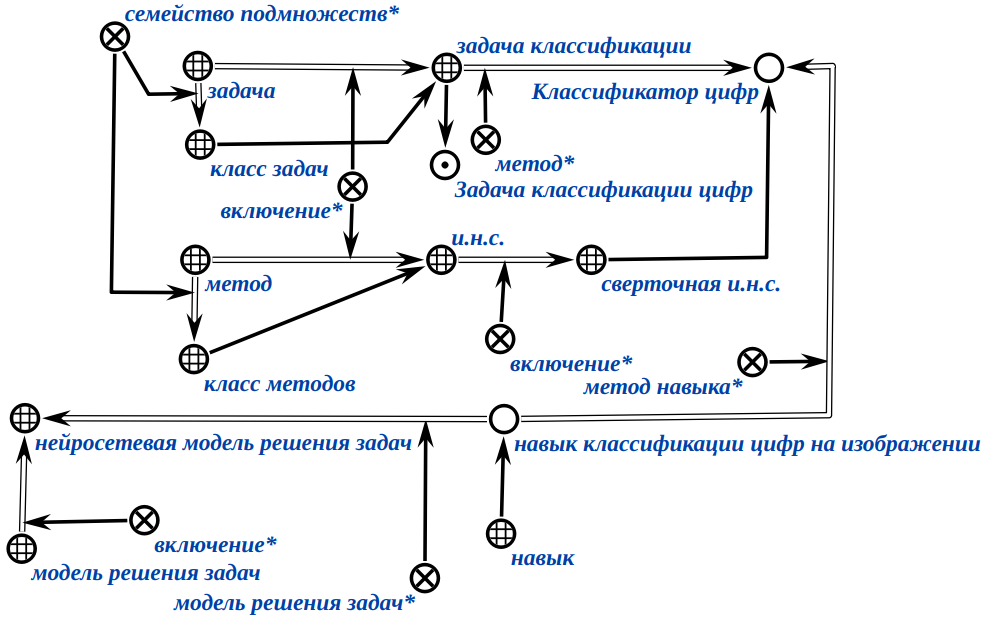
\includegraphics[scale=0.5]{author/part3/figures/actions_concepts.png}
	\caption{Фрагмент теоретико-множественной онтологии и.н.с.}
	\label{fig:actions_concepts}
\end{figure}

Использование и.н.с. как метода решения задач подразумевает использование уже спроектированной и обученной и.н.с. Однако наличие языка описания нейросетевого метода решения задач в памяти ostis-системы открывает дорогу для автоматизации самих процессов проектирования и обучения и.н.с. Такая автоматизация представляется отдельными классами задач и соответствующими навыками их решения. Подход к такой автоматизации описан в \textit{\ref{sec_chapter_ann_framework} \nameref{sec_chapter_ann_framework}}.

\subsection{Денотационная семантика моделей искусственных нейронных сетей, используемых в ostis-системах}

Как уже было сказано, денотационная семантика языка представления нейросетевого метода описывается в рамках предметной области (ПрО) и соответствующей ей онтологии нейросетевого метода. ПрО нейросетевого метода является дочерней ПрО метода.

Максимальным классом объектов исследования предметной области искусственных нейронных сетей является \textit{искусственная нейронная сеть}.

\begin{SCn}
	\scnheader{искусственная нейронная сеть}
	\scnidtf{и.н.с.}
	\scnidtf{нейросетевой метод}
	\scnidtf{множество искусственных нейронных сетей}
	\scnidtf{нейронная сеть}
	\scntext{пояснение}{Cовокупность нейронных элементов и связей между ними (см. \scncite{Golovko2017}).}
\end{SCn}

Искусственная нейронная сеть состоит из \textbf{\textit{формальных нейронов}}, которые связаны между собой посредством \textbf{\textit{синаптических связей}}. Нейроны организованы в \textbf{\textit{слои}}. Каждый нейрон слоя принимает сигналы со входящих в него синаптических связей, обрабатывает их единым образом с помощью заданной ему или всему слою \textbf{\textit{функции активации}} и передает результат на выходящие из него синаптические связи.

Архитектурой и.н.с. будем называть совокупность информации о структуре ее слоев, формальных нейронов, синаптических связей и функций активаций. Т.е. то, что можно обучить и использовать для решения задач.

Пример архитектуры и.н.с. представлен на рисунке \textit{\nameref{fig:nn_example}}.

\begin{figure}[H]
	\centering
	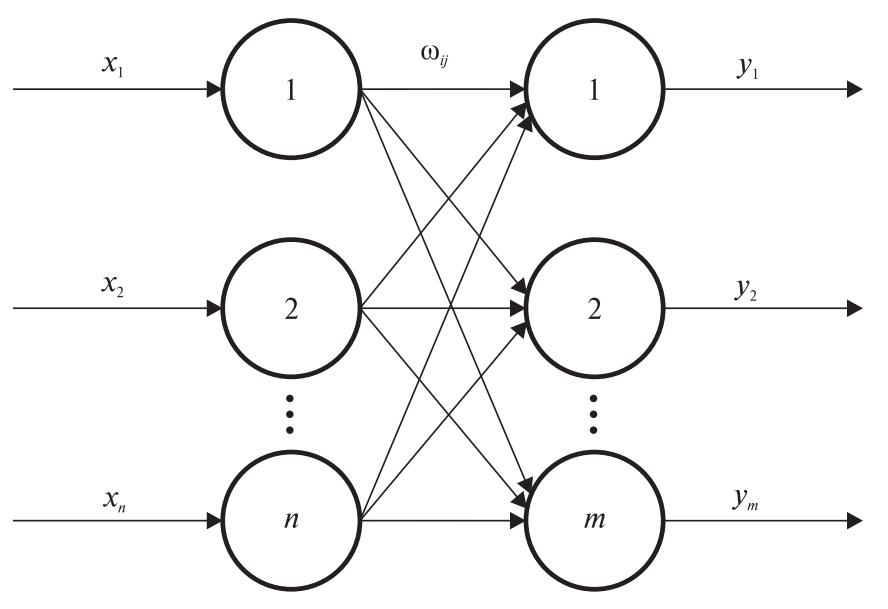
\includegraphics[scale=0.3]{author/part3/figures/neural_network.png}
	\caption{Пример архитектуры и.н.с.}
	\label{fig:nn_example}
\end{figure}

В соответствии с тем, какая у и.н.с. архитектура, можно выделить следующую иерархию классов и.н.с.. Рассмотрим эту иерархию в SCn-коде.

\begin{SCn}
	\scnheader{искусственная нейронная сеть}
	\scnidtf{нейросетевой метод}
	\scnrelto{включение}{метод}
	\scnrelfrom{разбиение}{Типология и.н.с. по признаку направленности связей\scnsupergroupsign}
	\begin{scnindent}
		\begin{scneqtoset}
			\scnitem{и.н.с. с прямыми связями}
			\begin{scnrelfromset}{декомпозиция}
				\scnitem{персептрон}
				\begin{scnrelfromset}{декомпозиция}
					\scnitem{персептрон Розенблатта}
					\scnitem{автоэнкодерная и.н.с.}
				\end{scnrelfromset}
				\scnitem{машина опорных векторов}
				\scnitem{и.н.с. сеть радиально-базисных функций}
				\scnitem{сверточная и.н.с.}
			\end{scnrelfromset}
			\scnitem{и.н.с. с обратными связями}
			\begin{scnrelfromset}{декомпозиция}
				\scnitem{и.н.с. Хопфилда}
				\scnitem{и.н.с. Хэмминга}
			\end{scnrelfromset}
			\scnitem{рекуррентная искусственная нейронная сеть}
			\begin{scnrelfromset}{декомпозиция}
				\scnitem{и.н.с. Джордана}
				\scnitem{и.н.с. Элмана}
				\scnitem{мультирекуррентная и.н.с.}
				\scnitem{LSTM-элемент}
				\scnitem{GRU-элемент}
			\end{scnrelfromset}
		\end{scneqtoset}
	\end{scnindent}
	\scnrelfrom{разбиение}{Типология и.н.с. по признаку полноты связей\scnsupergroupsign}
	\begin{scnindent}
		\begin{scneqtoset}
			\scnitem{полносвязная и.н.с.}
			\scnitem{слабосвязная и.н.с.}
		\end{scneqtoset}
	\end{scnindent}
\end{SCn}

Рассмотрим архитектурные компоненты подробнее.
\begin{SCn}
	\scnheader{формальный нейрон}
	\scnidtf{искусственный нейрон}
	\scnidtf{нейрон}
	\scnidtf{ф.н.}
	\scnidtf{нейронный элемент}
	\scnidtf{множество нейронов искусственных нейронных сетей}
	\scnidtf{математическая модель биологического нейрона}
	\scnsubset{искусственная нейронная сеть}
	\scntext{пояснение}{Основной элемент \textit{и.н.с.}, применяющий свою \textit{функцию активации} (см. \scncite{Golovko2017}) к сумме произведений входных сигналов на весовые коэффициенты:
		\begin{equation*}
			y = F\left(\sum_{i=1}^{n} w_ix_i - T\right) = F(WX - T)
		\end{equation*}
		где $X = (x_1,x_2,...,x_n)^{T}$ -- вектор входного сигнала; $W - (w_1,w_2,...,w_n)$ -- вектор весовых коэффициентов; \textit{T} -- пороговое значение;
		\textit{F} -- \textit{функция активации}.}
\end{SCn}

Отдельный формальный нейрон является искусственной нейронной сетью с одним нейроном в единственном слое.
Формальные нейроны могут быть классифицированы следующим образом:
\begin{textitemize}
	\item полносвязный формальный нейрон -- нейрон, у которого есть полный набор связей с нейронами предшествующего слоя. Oтдельный обрабатывающий элемент \textit{и.н.с.}, выполняющий функциональное преобразование взвешенной суммы элементов вектора входных значений с помощью \textit{функции активации};
	\item сверточный формальный нейрон -- отдельный обрабатывающий элемент \textit{и.н.с.}, выполняющий функциональное преобразование результата операции свертки матрицы входных значений с помощью \textit{функции активации}. Сверточный \textit{формальный нейрон} может быть представлен полносвязным \textit{формальным нейроном};
	\item рекуррентный \textit{формальный нейрон} -- нейрон, имеющий обратную связь с самим собой или с другими нейронами \textit{и.н.с.}
\end{textitemize}

Схематически формальный нейрон можно представить в виде следующей модели (рисунок \textit{\nameref{fig:formal_neuron}}).

\begin{figure}[H]
	\centering
	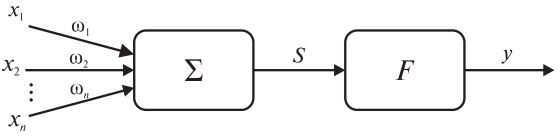
\includegraphics[scale=0.4]{author/part3/figures/formal_neuron.png}
	\caption{Формальный нейрон}
	\label{fig:formal_neuron}
\end{figure}

Определим понятия \textit{синаптической связи} и \textit{слоя и.н.с.}:

\begin{SCn}
	\scnheader{синаптическая связь}
	\scnidtf{синапс}
	\scnsubset{ориентированная пара}
	\scntext{пояснение}{ориентированная пара, первым компонентом которой является нейрон, из
	которого исходит сигнал, а вторым компонентом -- нейрон, который принимает этот сигнал}

	\scnheader{слой и.н.с.}
	\scnidtf{слой}
	\scnidtf{слой искусственной нейронной сети}
	\scnidtf{множество слоев искусственных нейронных сетей}
	\scnsubset{искусственная нейронная сеть}
	\scntext{пояснение}{множество нейронных элементов, на которые в каждый такт времени
	параллельно поступает информация от других нейронных элементов сети (см. \scncite{Golovko2017})}
	\scntext{пояснение}{множество формальных нейронов, осуществляющих параллельную независимую обработку вектора или матрицы входных значений}
\end{SCn}

Отдельный слой является искусственной нейронной сетью с одним слоем.
Следует отметить принципиальную важность этого замечания. Один \textit{слой и.н.с.}  уже является нейронной сетью, поскольку над ним можно производить все основные операции, которые производятся над "большой"{} \textit{и.н.с.} (его можно обучить и использовать для решения определенной задачи).

\textit{Слои и.н.с.} могут быть классифицированы следующим образом (по признаку операции, осуществляемой слоем):
\begin{textitemize}
	\item полносвязный слой и.н.с. -- слой, в котором каждый нейрон является полносвязным;
	\item сверточный слой и.н.с. -- слой, в котором каждый нейрон является сверточным;
	\item слой и.н.с. нелинейного преобразования -- слой, осуществляющий нелинейное преобразование входных данных;
	\item dropout слой и.н.с. -- слой, реализующий технику регуляризации dropout;
	\item pooling слой и.н.с. -- подвыборочный слой;
	\item слой и.н.с. батч-нормализации.
\end{textitemize}

Как правило, слой нелинейного преобразования выделяется в отдельный слой только в программных реализациях. Фактически он рассматривается как финальный этап расчета выходной активности любого нейрона -- применение \textit{функции активации}.

Dropout-слой функционирует только во время обучения \textit{и.н.с.}. Поскольку полносвязные слои имеют большое количество настраиваемых параметров, они подвержены эффекту \textit{переобучения}. Один из способов устранить такой негативный эффект -- выполнить частичный отсев результатов на выходе полносвязного слоя. На этапе обучения техника dropout позволяет отбросить выходную активность некоторых нейронов с определенной, заданной вероятностью. Выходная активность "отброшенных"{} нейронов полагается равной нулю.

Назначение подвыборочного слоя -- в осуществлении уменьшения размерности входных данных.

Нужно отметить, что данный перечень неполный -- разновидности \textit{слоев и.н.с.} появляются практически в каждой заслуживающей внимания публикации по нейросетевым алгоритмам и на текущий момент их существует достаточно много, однако, как правило, при построении более традиционных архитектур ограничиваются только приведенными вариантами слоев.

\textit{Слои и.н.с.} также могут быть классифицированы по исполняемой роли в рамках архитектуры (место в последовательности \textit{слоев и.н.с.}).

Так, например, слой, расположенный первым, называется распределяющим. Слои, расположенные далее, за исключением последнего, называются обрабатывающими. Наконец, последний слой носит название выходного \textit{слоя и.н.с.}

Последний архитектурный компонент \textit{и.н.с.} -- это функция активации:

\begin{SCn}
	\scnheader{функция активации*}
	\scnidtf{функция активации нейрона*}
	\scniselement{неролевое отношение}
	\scniselement{бинарное отношение}
	\scntext{пояснение}{неролевое отношение, связывающее формальный нейрон с функцией, результат
	применения которой к \textbf{\textit{взвешенной сумме нейрона}} определяет его \textbf{\textit{выходное значение}}.}
	\scnrelfrom{первый домен}{формальный нейрон}
	\scnrelfrom{второй домен}{функция}
\end{SCn}

Перечислим некоторые, наиболее известные и применяемые типы функций активации:
\begin{textitemize}
	\item линейная функция\\
	\scntext{формула}{
		\begin{equation*}
			y = kS
		\end{equation*}
		где \textit{k} -- коэффициент наклона прямой, \textit{S} -- в.с.
	};
	\item пороговая функция\\
	\scntext{формула}{
		\begin{equation*}
			y = sign(S) =
			\begin{cases}
				1, S > 0,\\
				0, S \leq 0
			\end{cases}
		\end{equation*}
	};
	\item сигмоидная функция\\
	\scntext{формула}{
		\begin{equation*}
			y = \frac{1}{1+e^{-cS}}
		\end{equation*}
		где \textit{с} > 0 -- коэффициент, характеризующий ширину сигмоидной функции по оси абсцисс, \textit{S} -- в.с.
	};
	\item функция гиперболического тангенса\\
	\scntext{формула}{
		\begin{equation*}
			y = \frac{e^{cS}-e^{-cS}}{e^{cs}+e^{-cS}}
		\end{equation*}
		где \textit{с} > 0 -- коэффициент, характеризующий ширину сигмоидной функции по оси абсцисс, \textit{S} -- в.с.
	};
	\item функция softmax\\
	\scntext{формула}{
		\begin{equation*}
			y_j = softmax(S_j) = \frac{e^{S_j}}{\sum_{j} e^{S_j}}
		\end{equation*}
		где $S_j$ -- в.с. \textit{j}-го выходного нейрона
	};
	\item функция ReLU\\
	\scntext{формула}{
		\begin{equation*}
			y = F(S) =
			\begin{cases}
				S, S > 0,\\
				kS, S \leq 0
			\end{cases}
		\end{equation*}
		где \textit{k} = 0 или принимает небольшое значение, например, 0.01 или 0.001.
	}
\end{textitemize}


В рамках предметной области формализована иерархия параметров и.н.с..
\begin{SCn}
	\scnheader{параметр и.н.с.}
	\scnsubset{параметр}
	\scnrelfrom{разбиение}{}
	\begin{scnindent}
		\begin{scneqtoset}
			\scnitem{настраиваемый параметр и.н.с.}
			\begin{scnrelfromset}{декомпозиция}
				\scnitem{весовой коэффициент синаптической связи}
				\scnitem{пороговое значение}
				\scnitem{ядро свертки}
			\end{scnrelfromset}
			\scnitem{архитектурный параметр и.н.с.}
			\begin{scnrelfromset}{декомпозиция}
				\scnitem{количество слоев}
				\scnitem{количество нейронов}
				\scnitem{количество синаптических связей}
			\end{scnrelfromset}
		\end{scneqtoset}
	\end{scnindent}
\end{SCn}

Так же в ПрО нейросетевых методов добавлены понятия для описания метрик эффективности нейросетевых методов. Данные метрики учитываются решателем задач при принятии решения об использовании того или иного нейросетевого метода.

Метрики могут быть классифицированы по типу решаемой задачи.
\begin{SCn}
	\scnheader{метрика оценки качества и.н.с.}
	\scnrelfrom{разбиение}{Типология метрик по признаку решаемой задачи\scnsupergroupsign}
	\begin{scnindent}
		\begin{scneqtoset}
			\scnitem{классификационные метрики}
			\begin{scnrelfromset}{декомпозиция}
				\scnitem{точность и.н.с.}
				\scnitem{полнота и.н.с.}
				\scnitem{F1-метрика}
			\end{scnrelfromset}
			\scnitem{регрессионные метрики}
			\begin{scnrelfromset}{декомпозиция}
				\scnitem{MAE}
				\scnitem{MAPE}
				\scnitem{RMSE}
			\end{scnrelfromset}
		\end{scneqtoset}
	\end{scnindent}

	\scnheader{точность и.н.с.}
	\scnidtf{precision}
	\scnidtf{доля верно идентифицированных положительных исходов в общем числе исходов, которые были идентифицированы как положительные}
	\scntext{формула}{
		\begin{equation*}
			PRE = \frac{TP}{TP + FP}
		\end{equation*}
		где \textit{TP} и \textit{FP} -- число истинно-положительных и ложно-положительных предсказаний нейронной сети соответственно
	}

	\scnheader{полнота и.н.с.}
	\scnidtf{recall}
	\scnidtf{доля верно идентифицированных положительных исходов в общем числе положительных исходов}
	\scntext{формула}{
		\begin{equation*}
			REC = \frac{TP}{TP + FN}
		\end{equation*}
		где \textit{TP} и \textit{FN} -- число истинно-положительных и ложно-отрицательных предсказаний нейронной сети соответственно
	}

	\scnheader{F1-метрика}
	\scntext{формула}{
		\begin{equation*}
			F1 = 2 * \frac{PRE * REC}{PRE + REC}
		\end{equation*}
		где \textit{PRE} и \textit{REC} -- точность и полнота и.и.с. соответственно
	}

	\scnheader{MAE}
	\scnidtf{mean absolute error}
	\scntext{формула}{$\frac{1}{N} \sum_{i=1}^N |y_{etalon}^i - y_{predicted}^i|$,\\ $y_{etalon}^i$ -- эталонное значение,\\ $y_{predicted}^i$ -- значение, полученное и.н.с.,\\ \textit{N} -- объем обучающей выборки
	}
\end{SCn}

\begin{SCn}
	\scnheader{MAPE}
	\scnidtf{mean absolute percentage error}
	\scntext{формула}{$\frac{1}{N} \sum_{i=1}^N \frac{|y_{etalon}^i - y_{predicted}^i|}{y_{etalon}^i} * 100\%$, \\ $y_{etalon}^i$ -- эталонное значение,\\ $y_{predicted}^i$ -- значение, полученное и.н.с.,\\ \textit{N} -- объем обучающей выборки
	}
\end{SCn}

\begin{SCn}
	\scnheader{RMSE}
	\scnidtf{root mean squared error}
	\scntext{формула}{$\sqrt{\frac{1}{N} \sum_{i=1}^N (y_{etalon}^i - y_{predicted}^i)^2}$, \\ $y_{etalon}^i$ -- эталонное значение,\\ $y_{predicted}^i$ -- значение, полученное и.н.с.,\\ \textit{N} -- объем обучающей выборки
	}
\end{SCn}

С помощью выделенных понятий становится возможна формализация в базе знаний архитектуры конкретных и.н.с.. В качестве примера, на рисунке \textit{\nameref{fig:neural_network_scg}} представлен пример формализации полносвязной двухслойной и.н.с. с двумя нейронами на входном слое и одном нейроне на обрабатывающем слоев.

\begin{figure}
	\centering
	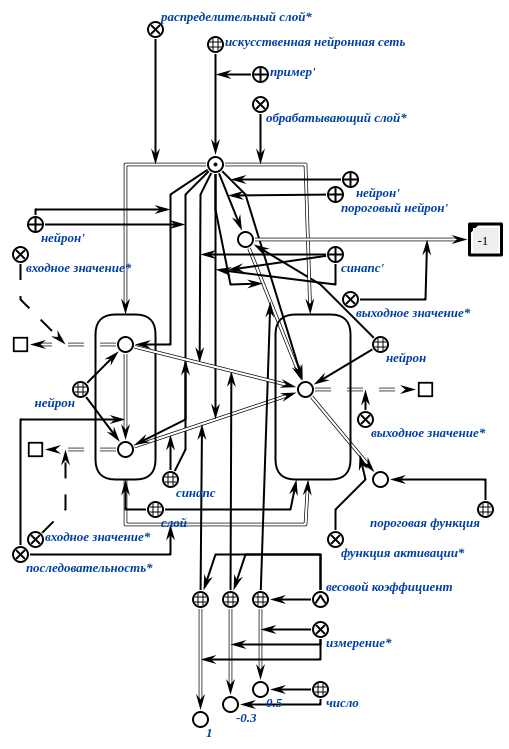
\includegraphics[width=0.8\linewidth]{author/part3/figures/neural_network_scg.png}
	\caption{Пример формализации архитектуры искусственной нейронной сети в базе знаний}
	\label{fig:neural_network_scg}
\end{figure}

Следует отметить, что в практике авторов еще не было необходимости явно представлять и.н.с., как это показано на рисунке \textit{\nameref{fig:neural_network_scg}}. Чаще всего, представление и.н.с. сводилось к представлению ее операционной семантики в виде SCP-программы, как это будет показано далее.

\subsection{Операционная семантика моделей искусственных нейронных сетей, используемых в ostis-системах}

Операционная семантика языка представления нейросетевого метода задается агентно-ориентированной моделью интерпретации искусственных нейронных сетей и спецификацией соответствующих действий.

Нейросетевой метод описан в виде программы на некотором языке программирования, который может быть как внешним по отношению к ostis-системе, так и внутренним (на данный момент, SCP). Каждому такому языку программирования соответствует некоторая дочерняя предметная область ПрО нейросетевых методов.

\begin{SCn}
	\scnheader{Предметная область нейросетевых методов}
	\scnidtf{Предметная область искусственных нейронных сетей}
	\begin{scnrelfromset}{дочерняя предметная область}
		\scnitem{Предметная область нейросетевых методов SCP}
		\scnitem{Предметная область нейросетевых методов Python}
		\scnitem{Предметная область нейросетевых методов C++}
	\end{scnrelfromset}
\end{SCn}

В случае описания нейросетевого метода на внешнем языке, такой метод описывается в соответствующей предметной области, в рамках которой также специфицируется действие интерпретации данного метода. Данному действию соответствует агент, реализованный на соответствующем языке программирования.

Однако для достижения конвергенции и интеграции необходимо описывать нейросетевые методы на внутреннем языке ostis-системы, которым является SCP.

SCP-программа является последовательностью обобщенных спецификаций (шаблонов) scp-операторов. Каждый scp-оператор является действием в памяти ostis-системы (sc-памяти). При интерпретации scp-программы, абстрактный sc-агент создания scp-процессов создает scp-процесс с учетом конкретных параметров интерпретации scp-программы, что на операционном уровне сводится к подстановке аргументов в обобщенные спецификации scp-операторов программы и генерации конкретных экземпляров этих программ(методов). Далее происходит добавление начального оператора во множество настоящих сущностей и начинается выполнение программы.

Таким образом, интерпретация scp-программы сводится к агентно-ориентированной обработке действий в sc-памяти. Этими действиями являются scp-операторы.

\begin{SCn}
	\scnheader{действие интерпретации слоя и.н.с.}
	\begin{scnrelfromset}{декомпозиция}
		\scnitem{действие вычисления взвешенной суммы всех нейронов слоя}
		\scnitem{действие вычисления функции активации всех нейронов слоя}
		\scnitem{действие интерпретации сверточного слоя}
		\scnitem{действие интерпретации пулинг слоя}
	\end{scnrelfromset}
\end{SCn}

Для описания спецификации указанных действий необходимо ввести понятия \textit{ориентированного множества чисел} и \textit{матрицы}, с помощью которых задаются входные значения и.н.с., выходные значения и.н.с., матрицы весовых коэффициентов и прочее.

Каждый элемент ориентированного множества чисел является некоторым числом. Числа могут быть представлены в виде sc-узлов, либо с помощью строкового представления всего множества, для чего используется специальное отношение \textit{строковое представление ормножества чисел*}, которое введено в целях оптимизации некоторых вариантов реализации агента, интерпретирующего действие, использующее понятие ориентированного множества чисел.

\begin{SCn}
	\scnheader{ориентированное множество чисел}
	\scnidtf{ормножество чисел}
	\scnrelto{включение}{число}
	\scnrelto{включение}{ориентированное множество}
	\scnrelto{первый домен}{строковое представление ормножества чисел*}
\end{SCn}

\textit{Матрица} является ориентированным множеством ориентированных множеств чисел равной мощности.


\textbf{1. Действие вычисления взвешенной суммы всех нейронов слоя}

Аргументы(\textit{объекты'}) этого действия задаются следующими отношениями:
\begin{SCn}
	\scnheader{входной вектор'}
	\scnrelfrom{первый домен}{действие интерпретации и.н.с.}
	\scnrelfrom{второй домен}{ориентированное множество чисел}
\end{SCn}

\begin{SCn}
	\scnheader{матрица весовых коэффициентов нейронов слоя'}
	\scnrelfrom{первый домен}{действие по обработке и.н.с.}
	\scnrelfrom{второй домен}{матрица}
\end{SCn}

Результатом действия(\textit{результат'}) является ориентированное множество чисел, являющихся взвешенной суммой нейронов соответствующего слоя.

Пример спецификации действия вычисления взвешенной суммы всех нейронов слоя для слоя с двумя нейронами и входным вектором размерностью 2 приведен на рисунке \textit{\nameref{fig:action_weighted_sum}}.

\begin{figure}
	\centering
	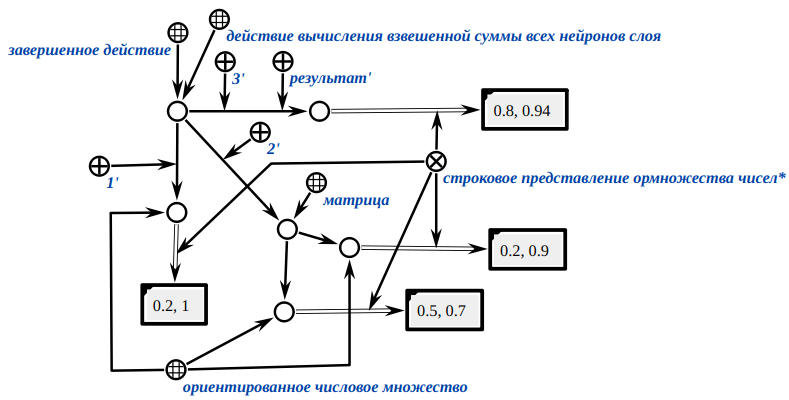
\includegraphics[width=0.95\linewidth]{author/part3/figures/action_weighted_sum.png}
	\caption{Пример действия вычисления взвешенной суммы всех нейронов слоя}
	\label{fig:action_weighted_sum}
\end{figure}


\textbf{2. Действие вычисления функции активации всех нейронов слоя}

Аргументы этого действия задаются следующими отношениями:
\begin{SCn}
	\scnheader{вектор взвешенных сумм нейронов слоя'}
	\scnrelfrom{первый домен}{действие по обработке и.н.с.}
	\scnrelfrom{второй домен}{ориентированное множество чисел}

	\scnheader{вектор порогов нейронов слоя'}
	\scnrelfrom{первый домен}{действие по обработке и.н.с.}
	\scnrelfrom{второй домен}{ориентированное множество чисел}

	\scnheader{функция активации'}
	\scnrelfrom{первый домен}{действие по обработке и.н.с.}
	\scnrelfrom{второй домен}{функция}
\end{SCn}

Результатом действия является ориентированное множество чисел, являющихся выходными значениями нейронов слоя.


\textbf{3. Действие интерпретации сверточного слоя}

Аргументы этого действия задаются следующими отношениями:
\begin{SCn}
	\scnheader{входная матрица'}
	\scnrelfrom{первый домен}{действие интерпретации и.н.с.}
	\scnrelfrom{второй домен}{матрица}

	\scnheader{ядро свертки'}
	\scnrelfrom{первый домен}{действие интерпретации сверточного слоя}
	\scnrelfrom{второй домен}{матрица}

	\scnheader{шаг свертки'}
	\scnrelfrom{первый домен}{действие интерпретации сверточного слоя}
	\scnrelfrom{второй домен}{число}
\end{SCn}

Результатом действия является матрица, полученная в результате свертки входной матрицы с ядром свертки.


\textbf{4. Действие интерпретации пулинг слоя}

Аргументы этого действия задаются следующими отношениями:
\begin{SCn}
	\scnheader{входная матрица'}
	\scnrelfrom{первый домен}{действие интерпретации и.н.с.}
	\scnrelfrom{второй домен}{матрица}

	\scnheader{размер окна пулинга'}
	\scnrelfrom{первый домен}{действие интерпретации пулинг слоя}
	\scnrelfrom{второй домен}{матрица}

	\scnheader{размер окна пулинга'}
	\scnrelfrom{первый домен}{действие интерпретации пулинг слоя}
	\scnrelfrom{второй домен}{матрица}

	\scnheader{шаг окна пулинга'}
	\scnrelfrom{первый домен}{действие интерпретации пулинг слоя}
	\scnrelfrom{второй домен}{число}
\end{SCn}

Результатом действия является матрица, полученная в результате пулинга входной матрицы.

При необходимости задавать различные аргументы для нейронов одного и того же слоя, можно специфицировать соответствующие действия, однако в этой работе этого не было произведено из-за слабой изученности подобного рода нейросетевых моделей.

Спецификация агентов, соответствующих указанным действиям, задает агентно-ориентированную модель интерпретации искусственных нейронных сетей. Реализация этой модели будет называться интерпретатором искусственных нейронных сетей

Рассмотрим пример описания на языке представления нейросетевого метода SCP, решающего задачу, которая формулируется следующим образом: вычислить результат логической операции ``ИСКЛЮЧАЮЩЕЕ ИЛИ'' для значений двух логических переменных. На рисунке \textit{\nameref{fig:strong_or_graphic}} представлено решение этой задачи с помощью сигнальной функции.

\begin{figure}
	\centering
	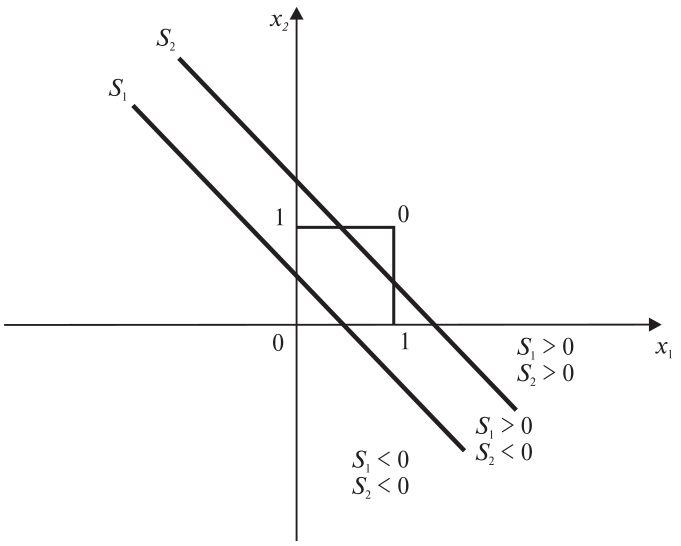
\includegraphics[width=0.5\linewidth]{author/part3/figures/strong_or_graphic.png}
	\caption{Решение задачи "ИСКЛЮЧАЮЩЕЕ ИЛИ"{}}
	\label{fig:strong_or_graphic}
\end{figure}

В работе \scncite{Golovko2017} описан однослойный персептрон, решающий поставленную задачу. Персептрон состоит из двух входных нейронов и одного выходного, с заданным порогом в 0,5 и сигнальной функцией активации:
\begin{equation*}
	F(S) =
	\begin{cases}
		1, 0 < S < 0,\\
		0, else
	\end{cases}
\end{equation*}

Весовые коэффициенты синапсов входного слоя равны 1. На рисунке \textit{\nameref{fig:strong_or_ann}} представлена схема персептрона.

\begin{figure}
	\centering
	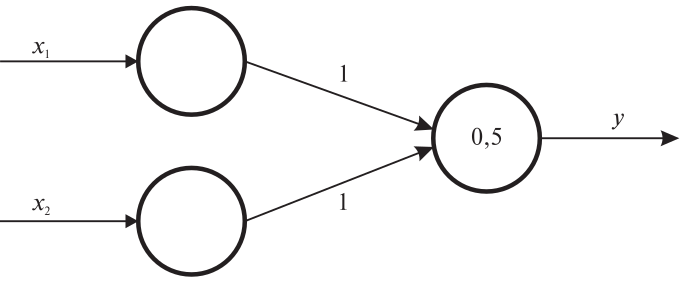
\includegraphics[width=0.5\linewidth]{author/part3/figures/strong_or_ann.png}
	\caption{Схема однослойного персептрона, решающего задачу "ИСКЛЮЧАЮЩЕЕ ИЛИ"{}}
	\label{fig:strong_or_ann}
\end{figure}

Данному персептрону соответствует метод, представленный в базе знаний ostis-системы на описанном в данной работе языке представления нейросетевых методов SCP. Данный метод представлен на рисунке \textit{\nameref{fig:exclusive_or_ann_scp}}.

\begin{figure}
	\centering
	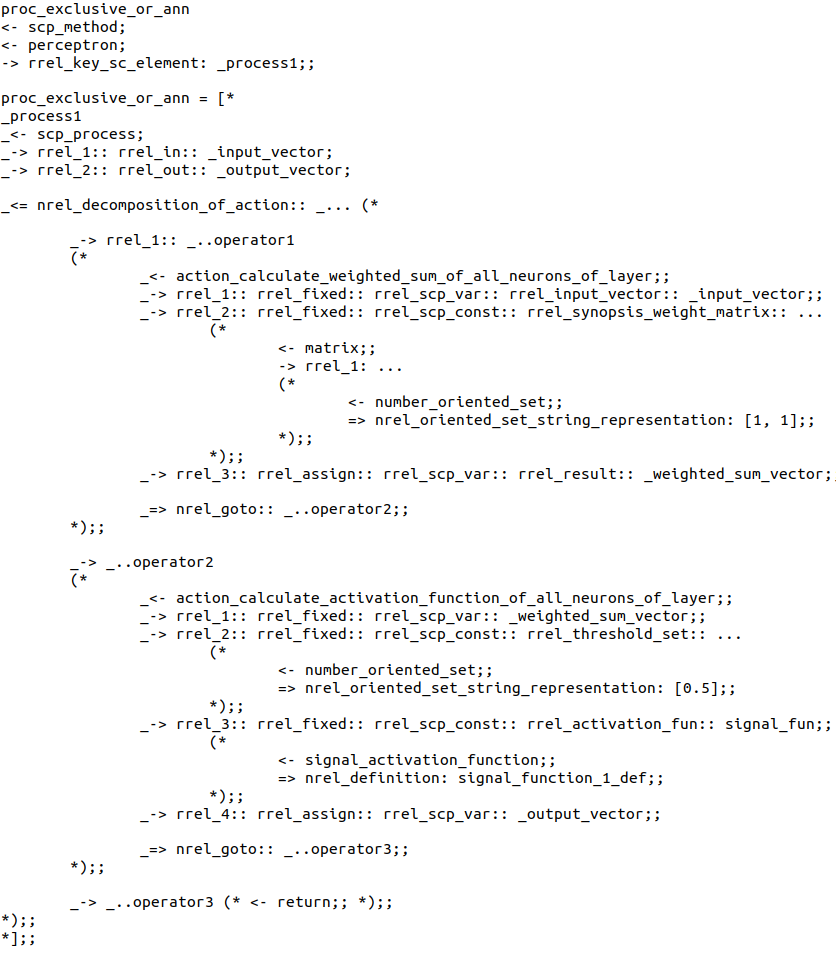
\includegraphics[width=0.95\linewidth]{author/part3/figures/exclusive_or_ann_scp.png}
	\caption{Метод, решающий задачу "ИСКЛЮЧАЮЩЕЕ ИЛИ"{}, представленный с помощью языка представления нейросетевых методов SCP}
	\label{fig:exclusive_or_ann_scp}
\end{figure}

Описание метода состоит из последовательности двух обобщенных спецификаций действий -- действия вычисления взвешенной суммы всех нейронов слоя и действия вычисления функции активации для всех нейронов слоя.

Сигнальная функция активации, использующаяся в персептроне, в памяти ostis-системы определяется логической формулой, представленной на рисунке \textit{\nameref{fig:signal_function_def}}.

\begin{figure}
	\centering
	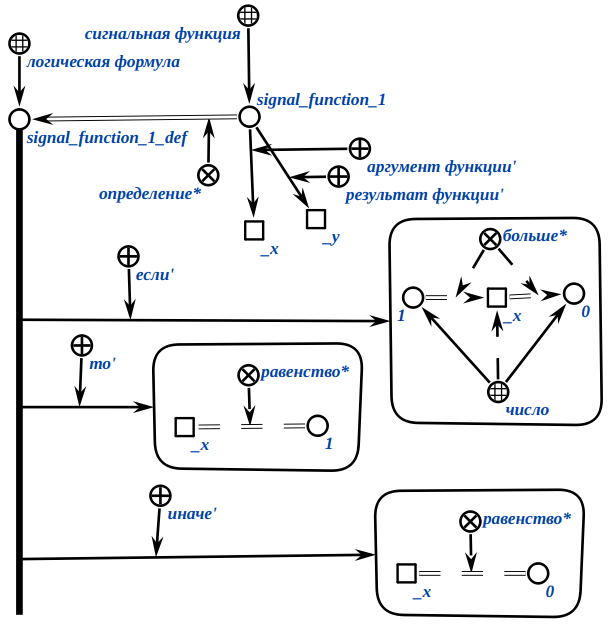
\includegraphics[width=0.5\linewidth]{author/part3/figures/signal_function_def.png}
	\caption{Представление сигнальной функции активации в памяти ostis-системы}
	\label{fig:signal_function_def}
\end{figure}

Любой агент, интерпретирующий действия с заданными с помощью отношения \textit{функция активации'} аргументами, должен использовать интерпретатор математических функций. использующихся в качестве функций активации.


\section{Логико-семантическая модель ostis-системы автоматизации проектирования искусственных нейронных сетей, семантически совместимых с базами знаний ostis-систем}
\label{sec_chapter_ann_framework}

Наличия языка представления нейросетевых методов SCP и его интерпретатора позволяет обеспечить интерпретацию нейросетевого метода в памяти ostis-системы. Наличие в единой памяти не только экземпляров методов, но и понятий, их описывающих, создает основу для автоматизации процесса построения нейросетевых методов. В памяти ostis-системы хранятся знания о том, методы какого класса могут решить задачу заданного класса, но экземпляров класса этого метода может не быть представлено в системе. На этот случай система должна иметь возможность сообщить пользователю о возможности решения, для которого, однако, необходимо погрузить в систему определенный метод. Так как система хранит в единой памяти задачу и требования к методу ее решения, появляется возможность спроектировать необходимый метод. Для этого необходимо наличие среды проектирования методов соответствующих классов. В случае нейросетевого метода, речь идет об интеллектуальной среде построения нейросетевых методов.

В основе интеллектуальной среды построения нейросетевых методов лежат соответствующие другу другу иерархии действий, задач и методов построения и.н.с. Наличие такой иерархии позволит описать язык представления методов построения и.н.с. и разработать интерпретатор этого языка.

Построение иерархии соответствующих действий построения и.н.с. следует начать с изучения этапов проектирования и обучения и.н.с., которые, в общем случае, выполняют все разработчики и.н.с.:


\textbf{1. Постановка задачи. }

Постановка задачи включает в себя описание входных данных (изображения/видео, временные ряды, текст), выходных данных и требований к методу решения (скорость, затраты по памяти и т.д.). Также описывается дополнительная информация, которая может помочь в построении метода решения задачи (к примеру, спецификация обучающей выборки, если таковая имеется). Обычно, на данном этапе разработчик и.н.с. определяет класс задачи, формирует требования к обучающей выборке, если она не предоставлена.

Выполнение данного этапа средой проектирования и.н.с. подразумевает выполнение следующих действий:
\begin{textitemize}
	\item \textit{Действие трансляции условия задачи}. Действие транслирует заданное с помощью интерфейса ostis-системы (к примеру, естественно-языкового интерфейса) описание задачи в память ostis-системы. Действие необходимо в случае, когда условие задачи задается пользователем. Необходимо понимать, что описание задачи поступает в базу знаний не только от пользовательского интерфейса. К примеру, задача может быть сформулирована самой системой в ходе ее жизнедеятельности.
	Данное действие является общим для всех ostis-систем, поэтому его рассмотрение выходит за рамки рассмотрения процесса построения интеллектуальной среды проектирования и.н.с.;
	\item \textit{Действие классификации задачи}. Действие определяет класс задачи (задача регрессии, детекции, кластеризации и т.д.), исходя из описания задачи в базе знаний;
	\item \textit{Действие поиска подходящей обучающей выборки}. В базе знаний может храниться набор спецификаций выборок, к которым у ostis-системы есть доступ. Действие производит поиск выборок, которые могут быть использованы в качестве обучающей выборки;
	\item \textit{Действие формирования требования к обучающей выборке}. Если обучающая выборка не была предоставлена и не была найдена, то необходимо сформировать описание требований к обучающей выборке, которое можно будет транслировать на язык пользовательского интерфейса и запросить необходимую выборку у пользователя.
\end{textitemize}


\textbf{2. Предобработка выборки: очистка}

На этом этапе обнаруживаются признаки, которые имеют в общем случае некорректные значения (например, для каких-то образов значение признака может иметь неопределенное значение, либо значение, не совпадающее по типу, либо аномально большое или очень маленькое значение, которое встречается в редком числе случаев). Для признаков, имеющих неопределенное значение, может быть применены различные методы устранения, например, такие значения могут быть заменены средним значением этого признака, рассчитанным по всем образам (для непоследовательных данных), либо они могут быть заменены средним значением по соседним образам (в случае временных рядов), либо каким-то фиксированным значением. Радикальная мера решения проблемы -- удаление образов, имеющих неопределенные значения признаков из выборки. Однако его лучше применять, если образов с отсутствующими значениями признаков немного. Для выбросов и аномалий применяются схожие стратегии (но только в том случае, если задача не состоит в прогнозировании этих аномалий).

В интеллектуальной среде проектирования данный этап соответствует выполнению \textbf{\textit{действия очистки выборки}}, которое выполняется в случае обработки выборки, которая ранее не была представлена в памяти системы (к примеру, была получена от пользователя).
Реализация интерпретатора (агента) данного действия требует описания в памяти классификации стратегий очистки данных и реализации методов применения этих стратегий.


\textbf{3. Предобработка выборки: выявление содержательных признаков}

Осуществляется т.н. инжиниринг признаков, состоящий в отборе признаков, влияющих на результат работы модели, несодержательные признаки, которые никак не коррелируют с выходом модели, удаляются. Цель этого этапа -- уменьшение размерности пространства признаков для снижения влияния эффекта переобучения на модель.

Для снижения размерности признакового пространства может применяться методы отбора признаков и выделения признаков.

При отборе признаков, осуществляется формирование подмножества из исходных признаков (алгоритм последовательного обратного отбора, рекурсивный алгоритм обратного устранения признаков,  алгоритмы с использованием случайных лесов).

При выделении признаков из набора признаков извлекается информация для построения нового подпространства признаков (алгоритмы с использованием автоэнкодера).

В интеллектуальной среде проектирования данный этап соответствует выполнению \textbf{\textit{действия выявления содержательных признаков}}. Реализация интерпретатора (агента) данного действия требует описания в памяти классификации стратегий уменьшения размерности признакового пространства и реализации методов применения этих стратегий.


\textbf{4. Предобработка выборки: трансформация}

На этом этапе осуществляется подготовка данных к обучению.
Здесь следует уделить особое внимание наличию категориальных признаков, чаще всего заданных строковыми типами. Эти признаки могут быть номинальными и порядковыми. Для кодирования порядковых признаков чаще всего применяют последовательный числовой код (1, 2, 3,...). Для кодирования номинальных такое решение неверно, т.к. эти признаки равноправны и не могут сравниваться по числовому коду (например, пол -- 0/1). Для номинальных признаков применяется способ прямого кодирования, заключающийся в создании и использовании фиктивных признаков по количеству значений исходного. Например, признак пол (мужской, женский) преобразуется в два новых признака мужской и женский с соответствующими значениями для имеющихся образов.

Масштабирование признаков предполагает приведение значений признаков к одному общему интервалу -- это особенно актуально для признаков, имеющих несоразмерные выборочные средние значения по всем образам -- например, один признак в среднем имеет значение 10.000, а другой 12. Это может проявится в выполнении минимизации только по признаку с наибольшими значениями и плохой сходимости метода обучения. Чаще всего масштабирование соответствует выполнению нормализации на отрезок (min-max нормализация):

\begin{equation*}
	x_{norm}^i = \frac{x^i - x_{min}}{x_{max} - x_{min}}
\end{equation*}
где $x^i$ -- значение признака для отдельно взятого образа \textit{i}, $x_{min}$ -- наименьшее значение для признака, $x_{max}$ -- наибольшее значение для признака.

Другой вариант масштабирования -- применение стандартизации признаков:

\begin{equation*}
	x_{std}^i = \frac{x^i - \mu(x)}{\sigma(x)},
\end{equation*}
$\mu(x)$ -- выборочное среднее отдельного признака, $\sigma(x)$ -- стандартное отклонение.

Стандартизация сохраняет полезную информацию о выбросах в исходных данных и делает алгоритм обучения менее чувствительным к ним.

Дискретизация применяется для перехода от вещественного признака к порядковому за счет кодирования интервалов одним значением (например, если признак отражает возраст человека, то может быть произведена дискретизация значений с выделением определенных возрастных групп, где каждая группа будет кодироваться одним целым числом).

В интеллектуальной среде проектирования данный этап соответствует выполнению \textbf{\textit{действия трансформации выборки}}. Реализация интерпретатора (агента) данного действия требует описания в памяти классификации методов масштабирования признаков и реализации методов применения этих стратегий.


\textbf{5. Разбиение выборки на обучающую, валидационную и тестовую (контрольную)}

Производится разбиение всей выборки данных, на обучающую, тестовую и, в некоторых случаях, валидационную.

Валидационная выборка используется для оценки влияния изменения гиперпараметров на результат обучения и может применяться как дополнительный инструмент для этого наравне с сеточным поиском.

Разбиение проводится в соотношении 3:1:1, в процентах (60/20/20), если валидационная выборка не используется, то 80/20.

В интеллектуальной среде проектирования данный этап соответствует выполнению \textbf{\textit{действия разбиения выборки}}.

Все предыдущие этапы применялись к выборке, последующие этапы относятся к используемым моделям и.н.с.


\textbf{6. Выбор класса нейросетевых методов в соответствии со сформулированной задачей}

На этом этапе осуществляется выбор основной архитектуры и.н.с., которая будет использоваться при обучении. Однако, нужно отметить, что этот выбор относительно условный, т.е. исследователь не ограничен использованием только одного типа и.н.с. для решения задачи (как, например, сверточной сети для изображений, поскольку изображения можно обрабатывать и обычным многослойным персептроном). Речь скорее идет именно о рекомендованной архитектуре, но это не исключает использование любых других вариантов архитектур и их сочетаний в рамках одной модели).

Примерами таких рекомендаций являются:
\begin{textitemize}
	\item Изображения/видео -- сверхточные нейронные сети;
	\item Временные ряды -- многослойные персептроны или рекуррентные сети;
	\item Текстовая информация -- многослойные персептроны или рекуррентные сети;
	\item Наборы характеристик некоторых объектов (например, спецификации автомобилей) -- многослойный персептрон.
\end{textitemize}

В интеллектуальной среде проектирования данный этап соответствует выполнению \textbf{\textit{действия выбора класса нейросетевых методов}}.


\textbf{7. Формирование спецификации на входные и выходные данные}

Выполняются дополнительные преобразования данных, связанные с изменением структур хранения (например, преобразование многомерного массива в одномерный, конвертация типов)

В интеллектуальной среде проектирования данный этап соответствует выполнению \textbf{\textit{действия формирования спецификации входов и выходов и.н.с.}}.


\textbf{8. Выбор метода оптимизации }

В рамках ПрО и.н.с. описаны следующие методы оптимизации:
\begin{textitemize}
	\item стохастический градиентный спуск (SGD);
	\item метод Нестерова;
	\item адаптивный градиент(AdaGrad);
	\item адаптивная оценка момента (Adam);
	\item среднеквадратическое распространение (RMSProp).
\end{textitemize}

В интеллектуальной среде проектирования данный этап соответствует выполнению \textbf{\textit{действия выбора метода оптимизации}}.


\textbf{9. Выбор минимизируемой функции ошибки}

На этом этапе задается функция ошибок, которая будет минимизироваться. К примеру, MSE лучше подходит для задач регрессии и для кластеризации, CE -- для классификационных задач.

Данные функции определяются следующим образом:
\begin{equation*}
	MSE = \frac{1}{n} \sum_{i=1}^n (Y_i - \widetilde{Y_i})^2
\end{equation*}
где \textit{n} -- размер обучающей выборки, $Y_i$ -- эталонное значение функции, $\widetilde{Y_i}$ -- результат, полученный НС

\begin{equation*}
	CE = - \frac{1}{n} \sum_{i=1}^n (Y_i\log(\widetilde{Y_i}) + (1-Y_i)\log(1 - \widetilde{Y_i}))
\end{equation*}
(случай 2-классовой классификации)

\begin{equation*}
	CE = - \frac{1}{n} \sum_{i=1}^n \sum_{c=1}^M Y_i^c \log{\widetilde{Y}_i^c}
\end{equation*}
(случай многоклассовой классификации)

В интеллектуальной среде проектирования данный этап соответствует выполнению \textbf{\textit{действия выбора минимизируемой функции ошибки}}.


\textbf{10. Начальная инициализация параметров нейронной сети}

Наиболее часто используемые варианты инициализации весовых коэффициентов и порогов нейронной сети включают:
\begin{textitemize}
	\item инициализация значениями из равномерного распределения на каком-то небольшом интервале, например, [-0.1, 0.1];
	\item инициализация значениями из стандартного нормального распределения;
	\item инициализация по методу Ксавье (см. \scncite{Glorot2010}).

	Применяется для предотвращения резкого уменьшения или увеличения значений выхода нейронных элементов после применения функции активации при прямом прохождении образа через глубокую нейронную сеть. Фактически инициализация этим методом осуществляется посредством выбора значений из равномерного распределения на отрезке $[- \sqrt{6} / \sqrt{n_i+n_{i+1}}, \sqrt{6} / \sqrt{n_i+n_{i+1}}]$, где $n_i$ -- это число входящих связей в данный слой, а $n_i$ -- число исходящих связей из данного слоя. Таким образом, инициализация этим методом проводится для разных слоев нейронной сети из разных отрезков;

	\item инициализация, полученная из предобученной модели.

	Вариант инициализации, который предполагает использование в качестве "стартовой"{} модели предобученной модели, взятой из некоторого репозитория предобученных моделей, обученную самим исследователем или в процессе работы интеллектуальной системы;

	\item инициализация по методу Кайминга (см. \scncite{He2015}).

	Данный метод инициализации применяется для решения проблемы "затухающего"{} градиента и "взрывающегося"{}
	градиента. Производится посредством выбора значений из равномерного распределения на отрезке $[-\sqrt{2} / \sqrt{(1+a^2)fan}, \sqrt{2} / \sqrt{(1+a^2)fan}]$,
	где \textit{a} -- угол наклона к оси абсцисс для отрицательной части области определения функции активации типа ReLU (для обычной ReLU функции этот параметр равен 0), $fan$ -- параметр режима работы, который для фазы прямого распространения равен количеству входящих связей (для устранения эффекта "взрывающегося"{} градиента), а для фазы обратного распространения -- количеству выходящих (для устранения эффекта "затухающего"{} градиента).
\end{textitemize}

В интеллектуальной среде проектирования данный этап соответствует выполнению \textbf{\textit{действия начальной инициализации и.н.с.}}.


\textbf{11. Выбора гиперпараметров и.н.с.}

На практике некоторые гиперпараметры (такие как количество слоев, их типы, количество нейронов в слое) часто определяются экспериментально, в процессе итеративного поиска лучшего варианта решения задачи. Хотя способы частично автоматизировать этот процесс существуют, они все же рассчитаны на наличие некоторых предусловий проведения эксперимента, в частности интервалов изменения параметра (например, скорости обучения).

К гиперпараметрам, подбираемым на этом этапе, относятся:
\begin{textitemize}
	\item Параметры обучения и.н.с. (скорость обучения, моментный параметр, размер мини-батча);
	\item Архитектура модели и.н.с., опирающаяся на ранее сформулированные спецификации входных и выходных данных (например, количество нейронов в определенном слое (слоях) или конфигурации целых слоев).
\end{textitemize}

Нахождение оптимальных гиперпараметров может быть получено, например, использованием метода сеточного поиска, который позволяет проверить значения гиперпараметров, взятые с определенным шагом или из определенного интервала (кортежа). С помощью этого метода выбирается оптимальный набор гиперпараметров, который дает лучшие результаты, он используется для последующего дообучения. Или же, если полученные результаты являются приемлемыми, то процесс дальнейшего обучения вообще не проводится. Следует отметить затратность данного метода, т.к. фактически осуществляется перебор различных значений параметров обучения. Для снижения объема работы применяется метод случайного поиска.

Для оптимизации архитектуры определяются типы слоев нейронной сети, количество нейронных элементов в каждом слое, их характеристики -- функция активации, для сверточных элементов -- размер ядра, а также параметры padding и шаг свертки (stride).
Здесь же может осуществляться оценка не только пользовательского варианта сети, но и предобученной архитектуры. Основное правило при выборе -- количество параметров модели не должно превышать размер обучающей выборки. Для предобученных архитектур это ограничение снимается.

В интеллектуальной среде проектирования данный этап соответствует выполнению \textbf{\textit{действия выбора гипперпараметров и.н.с.}}. Действие использует классификацию и спецификации гиперпараметров и.н.с..


\textbf{12. Обучение модели на обучающей выборке}

Производится обучение модели до достижения выбранной точности (оценивается на тестовой выборке) или по другим заданным критериям (достижение заданного количества эпох обучения, неизменность точности на протяжении заданного количества эпох, падение точности на валидационной выборке и т.д.)

Приведем классификацию алгоритмов обучения:
\begin{SCn}
	\scnheader{метод обучения и.н.с.}
	\scnsubset{метод}
	\scnsuperset{метод обучения с учителем}
	\begin{scnindent}
		\scntext{explanation}{
			\textbf{\textit{метод обучения с учителем}} -- метод обучения с использованием заданных целевых переменных.
		}
		\scnsuperset{метод обратного распространения ошибки}
		\begin{scnindent}
			\scnidtf{м.о.р.о.}
			\scntext{explanation}{м.о.р.о. использует заданный метод оптимизации и заданную функцию потерь для реализации фазы обратного распространения ошибки и изменения настраиваемых параметров и.н.с. Одним из самых распространенных
			методов оптимизации является метод стохастического градиентного спуска.
			}
			\scntext{explanation}{Следует также отметить, что несмотря на то, что метод отнесен к методам обучения с учителем, в случае
			использования м.о.р.о. для обучения автокодировщиков в классических публикациях он рассматривается как
			метод обучения без учителя, поскольку в данном случае размеченные данные отсутствуют.
			}
		\end{scnindent}
	\end{scnindent}
	\scnsuperset{метод обучения без учителя}
	\begin{scnindent}
		\scntext{explanation}{\textbf{\textit{метод обучения без учителя}} -- метод обучения без использования заданных целевых переменных(в режиме самоорганизации)
		}
		\scntext{explanation}{В ходе выполнения алгоритма метода обучения без учителя выявляются полезные структурные свойства
		набора. Неформально его понимают как метод для извлечения информации из распределения, выборка для которого
		не была вручную аннотирована человеком (см. \scncite{Goodfellow2017}).
		}
	\end{scnindent}
\end{SCn}

В интеллектуальной среде проектирования данный этап соответствует выполнению \textbf{\textit{действия обучения и.н.с.}}. Действие обучения  \textit{и.н.с.} -- действие, в ходе которого реализуется определенный метод обучения  \textit{и.н.с.} с заданными параметрами обучения  \textit{и.н.с.}, методом оптимизации и функцией потерь.

При обучении возможно возникновение следующих проблем:

\begin{textitemize}
	\item Переобучение -- проблема, возникающая при обучении  \textit{и.н.с.}, заключающаяся в том,
	что сеть хорошо адаптируется к паттернам входной активности из обучающей выборки, при этом теряя способность к обобщению.
	Переобучение возникает из-за применения неоправданно сложной модели при обучении  \textit{и.н.с.} Это происходит,
	когда количество настраиваемых параметров и.н.с. намного больше размера обучающей выборки. Возможные
	варианты решения проблемы заключаются в упрощении модели, увеличении выборки, использовании регуляризации
	(параметр регуляризации, техника dropout и т.д.).\\
	Обнаружение переобученности сложнее, чем недообученности. Как правило, для этого применяется
	кросс-валидация на валидационной выборке, позволяющая оценить момент завершения процесса обучения.
	Идеальным вариантом является достижение баланса между переобученностью и недообученностью;

	\item Недообучение -- проблема, возникающая при обучении  \textit{и.н.с.}, заключающаяся в том,
	что сеть дает одинаково плохие результаты на обучающей и контрольной выборках.
	Чаще всего такого рода проблема возникает при недостаточном времени, затраченном на обучение модели.
	Однако это может быть вызвано и слишком простой архитектурой модели либо малым размером обучающей
	выборки. Соответственно решение, которое может быть принято ML-инженером, заключается в устранении
	этих недостатков: увеличение времени обучения, использование модели с большим числом настраиваемых
	параметров, увеличение размера обучающей выборки, а также уменьшение регуляризации и более тщательный
	отбор признаков для обучающих примеров.
\end{textitemize}

Методом обучения \textit{и.н.с.} называется процесс итеративного поиска оптимальных значений настраиваемых параметров и.н.с., минимизирующих некоторую заданную функцию потерь.

Стоит отметить, что хотя целью применения метода обучения является минимизация функции потерь, "полезность"{} полученной после обучения модели можно оценить только по достигнутому уровню ее обобщающей способности.

Методы обучения могут быть поделены на две большие группы -- \textit{\textbf{методы обучения с учителем}} и \textit{\textbf{методы обучения без учителя}} (контролируемый и неконтролируемый методы обучения).

Метод обучения с учителем -- метод обучения с использованием заданных целевых переменных.

Одним из методов обучения с учителем является метод обратного распространения ошибки.

Приведем его описание в виде алгоритма:

\begin{algorithm}[H]
	\KwData{$X$ -- данные, $E_t$ -- желаемый отклик (метки), $E_m$ -- желаемая ошибка (в соответствии с выбранной функцией потерь)}
	\KwResult{обученная нейронная сеть \textit{Net}}
	инициализация весов \textit{W} и порогов \textit{T};\\
	\Repeat{$E<E_m$}{
		\ForEach{$x \in X$, $e \in E_t$}{
			фаза прямого распространения сигнала: вычисляются активации для всех слоев и.н.с.;\\
			фаза обратного распространения ошибки: вычисляются ошибки для последнего слоя и всех предшествующих слоев;\\
			изменение настраиваемых параметров и.н.с. в соответствии с вычисленными ошибками;\\
		}
		вычисление общей ошибки E на данной эпохе;
	}
\end{algorithm}

Метод обратного распространения ошибки использует заданный метод оптимизации и заданную функцию потерь для реализации фазы обратного распространения ошибки и изменения настраиваемых параметров и.н.с. Одним из самых распространенных методов оптимизации является метод стохастического градиентного спуска. Приведенный метод используется для реализации последовательного варианта обучения.

Следует также отметить, что несмотря на то, что метод отнесен к методам обучения с учителем, в случае
его использования для обучения автокодировщиков в классических публикациях он рассматривается как
метод обучения без учителя, поскольку в данном случае размеченные данные отсутствуют.

\textbf{\textit{Метод обучения без учителя}} -- метод обучения без использования заданных целевых переменных (в режиме самоорганизации)

В ходе выполнения алгоритма метода обучения без учителя выявляются полезные структурные свойства
набора. Неформально его понимают как метод для извлечения информации из распределения, выборка для которого
не была вручную аннотирована человеком (см. \scncite{Goodfellow2017}). Метод обучения без учителя может рассматриваться как вспомогательный метод для начальной инициализации настраиваемых параметров и.н.с. В этом случае он является методом предобучения.

Среди методов, применяемых для оптимизации целевой функции можно выделить следующие:

\begin{textitemize}
	\item SGD (стохастический градиентный спуск): в данном методе корректировка настраиваемых параметров и.н.с. выполняется в направлении максимального уменьшения функции стоимости, т.е. в направлении, противоположном вектору градиента функции потерь (см. \scncite{Haykin2006});
	\item метод Нестерова: Обучение методом стохастического градиентного спуска иногда происходит очень медленно. Импульсный метод позволяет ускорить обучение, особенно в условиях высокой кривизны, небольших, но устойчивых градиентов или зашумленных градиентов. В импульсном методе вычисляется экспоненциально затухающее скользящее среднее прошлых градиентов и продолжается движение в этом направлении. Метод Нестерова является вариантом импульсного алгоритма, в котором градиент вычисляется после применения текущей скорости (см. \scncite{Goodfellow2017});
	\item AdaGrad: Данный метод по отдельности адаптирует скорости обучения всех настраиваемых параметров и.н.с., умножая их на коэффициент, обратно пропорциональный квадратному корню из суммы всех прошлых значений квадрата градиента (см. \scncite{Duchi2011});
	\item RMSProp: Данный метод является модификацией AdaGrad, которая позволяет улучшить его поведение в невыпуклом случае путем изменения способа агрегирования градиента на экспоненциально взвешенное скользящее среднее. Использование экспоненциально взвешенного скользящего среднего гарантирует повышение скорости сходимости после обнаружения выпуклой впадины, как если бы внутри этой впадины алгоритм AdaGrad был инициализирован заново (см. \scncite{Goodfellow2017});
	\item Adam: Данный метод можно рассматривать как комбинацию RMSProp и AdaGrad (см. \scncite{Kingma2014}). Помимо усредненного первого момента, данный метод использует усредненное значение вторых моментов градиентов.
\end{textitemize}

Отметим, что успешность применения методов оптимизации зависит главным образом от знакомства пользователя с соответствующим алгоритмом (см. \scncite{Goodfellow2017}).

Еще одним важным компонентом, влияющим на процесс обучения, является используемая функция потерь.

\textit{Функция потерь} -- функция, используемая для вычисления ошибки, рассчитываемой как разница между фактическим эталонным значением и прогнозируемым значением, получаемым \textit{и.н.с.}

Среди функций потерь, используемые в качестве целевых функций для применяемого метода оптимизации, можно выделить:

\begin{textitemize}
	\item MSE -- средняя квадратичная ошибка\\
	\begin{equation*}
		MSE = \frac{1}{L} \sum_{l=1}^L \sum_{i=1}^m (y_i^l - e_i^l)^2
	\end{equation*}
	где $y_i^l$ -- прогноз модели, $e_i^l$ -- ожидаемый (эталонный) результат, \textit{m} -- размерность выходного вектора, \textit{L} -- объем обучающей выборки;

	\item BCE -- бинарная кросс-энтропия\\
	\begin{equation*}
		BCE = - \sum_{l=1}^L (e^l \log(y^l) + (1 - e^l)\log(1 - y^l))
	\end{equation*}
	где $y^l$ -- прогноз модели, $e^l$ -- ожидаемый (эталонный) результат: \textit{0} или \textit{1}, \textit{L} -- объем обучающей выборки;
	\item MCE -- мультиклассовая кросс-энтропия\\
	\begin{equation*}
		MCE = - \sum_{l=1}^L \sum_{i=1}^m e_{i}^l \log(y_{i}^l)
	\end{equation*}
	где $y_{i}^l$ -- прогноз модели, $e_i^l$ -- ожидаемый (эталонный результат), \textit{m} -- размерность выходного вектора.
\end{textitemize}

Отметим, что для бинарной кросс-энтропии в выходном слое \textit{и.н.с.} будет находиться один нейрон, а для для мультиклассовой кросс-энтропии количество нейронов в выходном \textit{слое и.н.с.} совпадает с количеством классов.

Для решения задачи классификации рекомендуется использовать бинарную или мультиклассовую кросс-энтропийную функцию потерь, для решения задачи регрессии рекомендуется использовать среднюю квадратичную ошибку.

Действие обучения \textit{и.н.с.} можно проиллюстрировать следующим изображением \textit{\nameref{fig:ann_training_nn_scg}}.

\begin{figure}[H]
	\centering
	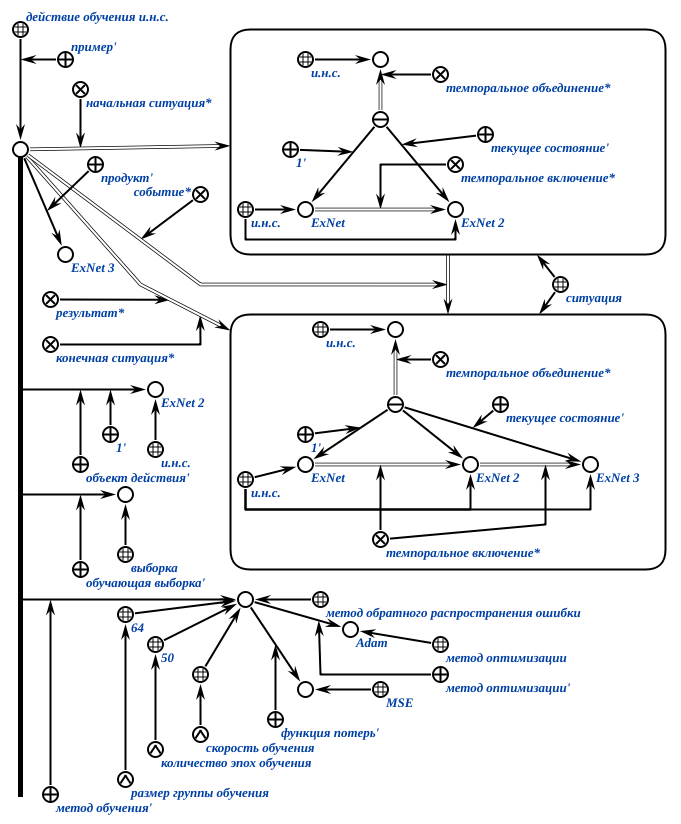
\includegraphics[scale=0.7]{author/part3/figures/ann_training_nn_scg.png}
	\caption{Действие обучения и.н.с.}
	\label{fig:ann_training_nn_scg}
\end{figure}

\textbf{13. Оценка эффективности и.н.с}

После выполнения обучения осуществляется оценка полученной модели с помощью метрик оценки качества.

Далее результат оценки может быть визуализирован с помощью матрицы ошибок (confusion matrix) и ROC-кривой.

Матрица ошибок представляется собой матрицу (рис. \nameref{fig:conf_matrix}), в которую помещены сведения о числе истинно-положительных, истинно-отрицательных, ложно-положительных и ложно-отрицательных предсказаниях классификатора.

\begin{figure}[h]
	\centering
	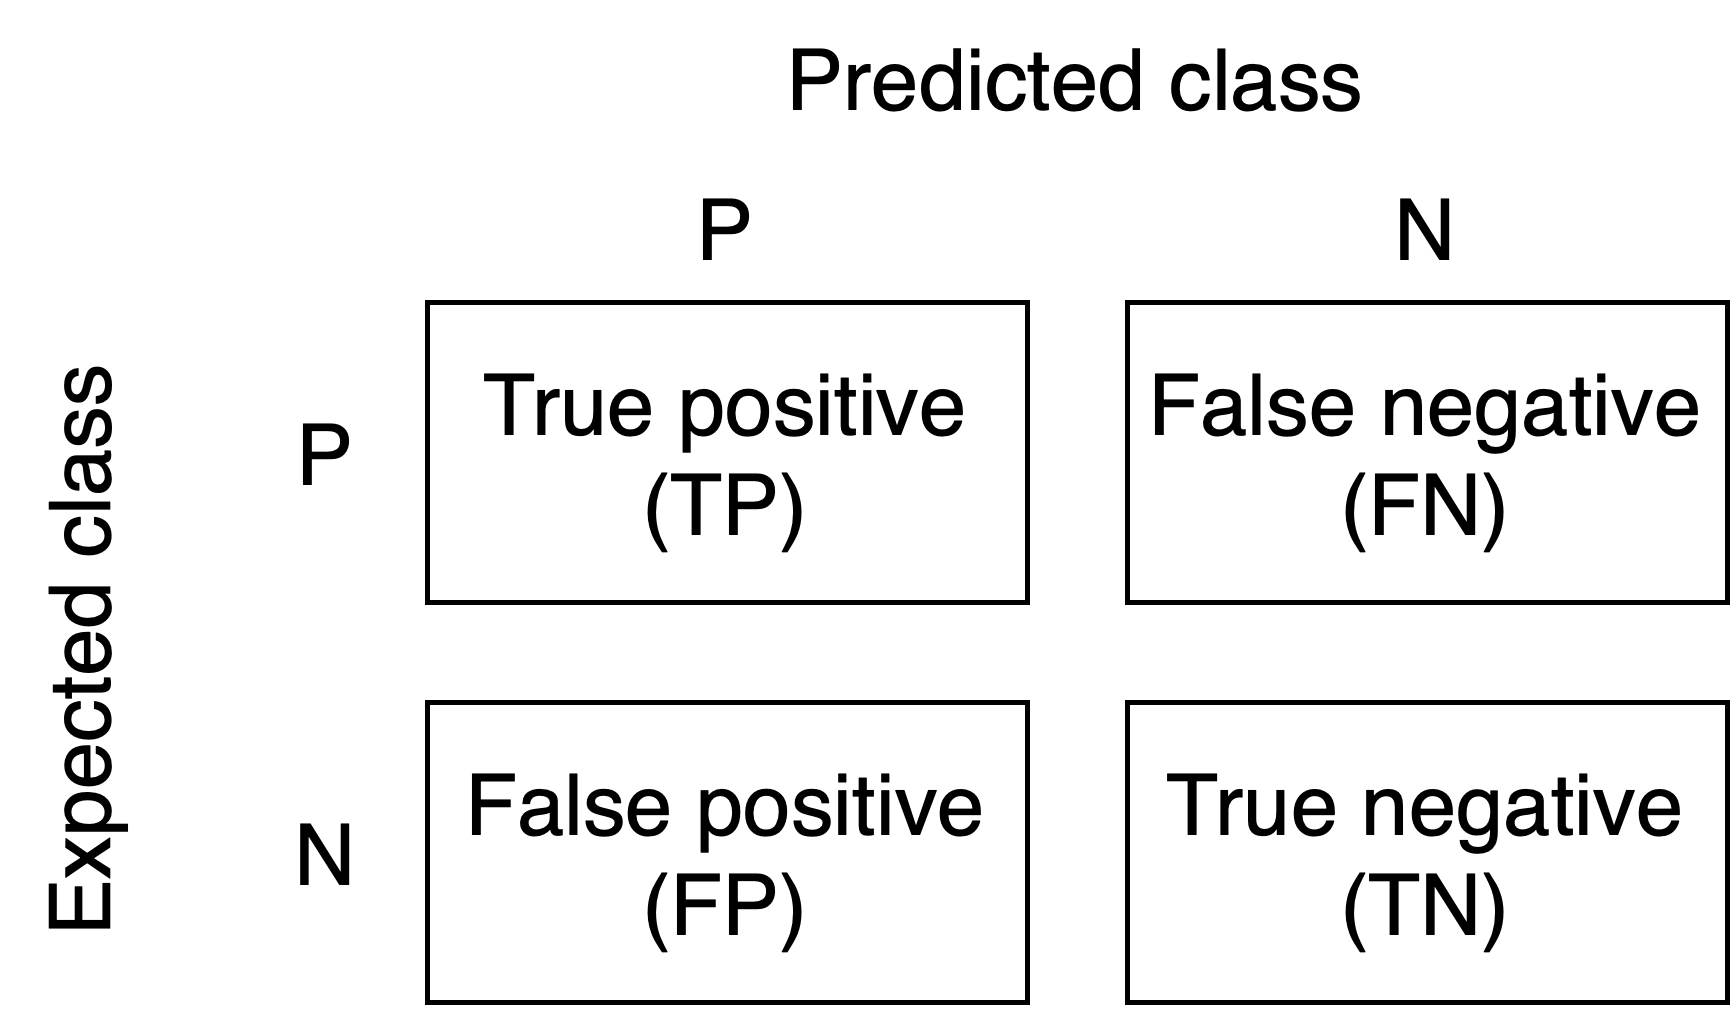
\includegraphics[width=0.4\textwidth]{author/part3/figures/conf_matrix.png}
	\caption{Матрица ошибок}
	\label{fig:conf_matrix}
\end{figure}

ROC-кривая -- это график, в котором, основываясь на заданном пороге решения классификатора, рассчитываются доли ложноположительных и истинно положительных исходов. Основываясь на ROC-кривой, высчитывается AUC-показатель (площадь под кривой), которая используется в качестве характеристики качества модели.

В интеллектуальной среде проектирования данный этап соответствует выполнению \textit{действия оценки эффективности и.н.с.}.

Рассмотрим пример выполнения описанных этапов разработчиком для конкретной задачи -- \textit{классификации цифр из выборки рукописных цифр MNIST}:


\textbf{1.} Исходными данными задачи является: выборка из 70.000 изображений, предварительно разделенная на обучающую (60.000 изображений) и контрольную (10.000 изображений) выборки. Каждое изображение представлено двумерным массивом 28Х28 чисел из интервала [0, 255], числа представляют определенный оттенок серого цвета. Помимо этого каждому изображению соответствует метка класса, соответствующая конкретной цифре от 0 до 9.

Ставится задача: \textit{обучить модель, которая будет принимать на вход двумерный массив данных и возвращать метку класса, соответствующей распознанной цифре.}

Таким образом, тип решаемой задачи -- \textbf{классификационная}, природа данных задачи -- \textbf{изображения}.


\textbf{2.} В рассматриваемой выборке отсутствуют аномалии, ошибочные данные, признаки с отсутствующими значениями.


\textbf{3.} В рассматриваемой задаче отсутствуют несодержательные признаки.


\textbf{4.} В качестве метода предобработки данных используем масштабирование признаков, а именно нормализацию на отрезок [0, 1].


\textbf{5.} Выполним разбиение обучающей части данных на обучающую и валидационную выборки в соотношении 4:1 (48.000 в обучающей и 12.000 в валидационной).


\textbf{6.} Так как выборка включает в себя изображения, будем использовать сверточную нейронную сеть.


\textbf{7.} Не требуется.


\textbf{8.} В качестве оптимизационного алгоритма будем использовать метод стохастического градиентного спуска (SGD).


\textbf{9.} Так как решается задача классификации, выберем в качестве минимизируемой функции кросс-энтропийную функцию потерь.


\textbf{10.} В качестве начальной инициализации будем использовать инициализацию по методу Кайминга.


\textbf{11.} На этапе 6 и 8 было определено, что для решения задачи будет использоваться сверточная нейронная сеть. При использовании one-hot кодирования в последнем полносвязном слое будет 10 нейронов по числу классов в задаче.

Для упрощения будем использовать архитектуру, изображенную на рис. \nameref{fig:model}, не содержащую промежуточные слои.

\begin{figure}[h]
	\centering
	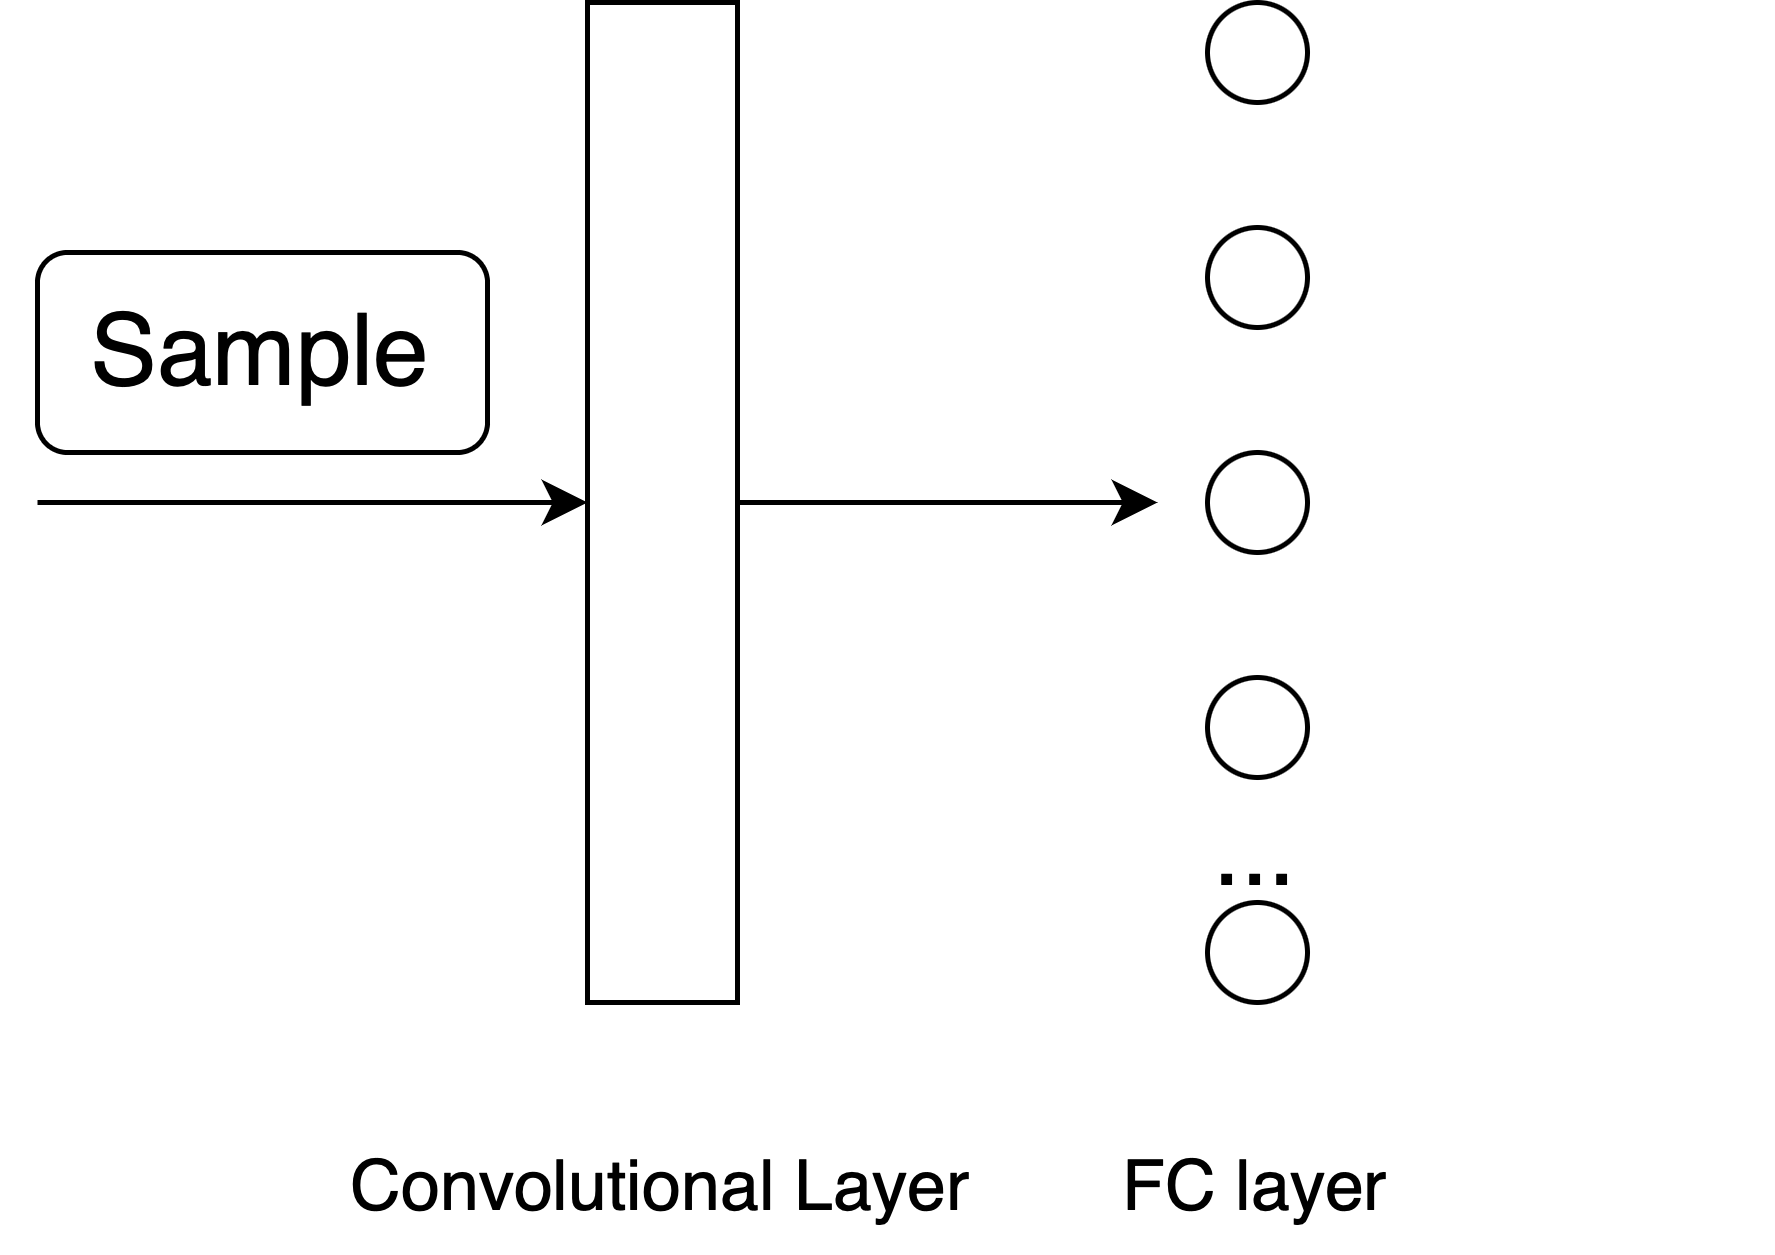
\includegraphics[width=0.4\textwidth]{author/part3/figures/model.png}
	\caption{Архитектура и.н.с., решающая задачу классификации цифр}
	\label{fig:model}
\end{figure}

Для нахождения оптимального набора гиперпараметров будем применять метод случайного поиска.

Перечислим кортежи, из которых будут сэмплироваться гиперпараметры:
\begin{textitemize}
	\item Скорость обучения -- (0.9, 0.1, 0.01, 0.001);
	\item Количество нейронов в сверточном слое -- (5, 10, 15, 20);
	\item Размер ядра свертки -- (3, 5, 7, 9);
	\item Моментный параметр -- (0, 0.5, 0.9);
	\item Размер мини-батча -- (16, 32, 64, 128).
\end{textitemize}

После определения данных параметров и оценки эффективности работы алгоритма, получим следующую таблицу:

\begin{table}[ht]
	\caption{Результаты решения задачи \\(используемые сокращения: mbs -- mini-batch size, ks -- kernel size, lr -- learning rate, cnc -- convolutional neurons count, acc -- accuracy, it -- iterations count)}
	\centering
	\begin{tabular}{c c c c c c c c}
		\hline\hline
		\# & mbs & ks & lr    & momentum & cnc & acc    & it \\ [0.5ex] % inserts table %heading
		\hline
		1        & 128 & 3  & 0.001 & 0.5      & 10  & 0.9033 & 10 \\
		2        & 64  & 9  & 0.9   & 0        & 15  & 0.1039 & 1  \\
		3        & 32  & 3  & 0.01  & 0.5      & 20  & 0.9741 & 10 \\
		4        & 32  & 7  & 0.01  & 0.5      & 15  & 0.9794 & 10 \\
		5        & 16  & 9  & 0.001 & 0.5      & 20  & 0.9189 & 2  \\
		6        & 64  & 3  & 0.1   & 0.5      & 10  & 0.9736 & 10 \\
		7        & 64  & 7  & 0.001 & 0.9      & 15  & 0.9007 & 1  \\
		8        & 32  & 9  & 0.1   & 0.5      & 5   & 0.9806 & 10 \\
		9        & 128 & 5  & 0.1   & 0.5      & 20  & 0.98   & 10 \\
		10       & 32  & 9  & 0.01  & 0.9      & 5   & 0.9806 & 10 \\
		11       & 128 & 3  & 0.001 & 0.9      & 10  & 0.893  & 1  \\
		12       & 32  & 5  & 0.9   & 0.9      & 20  & 0.1008 & 1  \\
		13       & 16  & 9  & 0.9   & 0.5      & 20  & 0.0976 & 1  \\
		14       & 32  & 7  & 0.9   & 0.9      & 15  & 0.0932 & 1  \\
		15       & 128 & 5  & 0.01  & 0.5      & 20  & 0.9197 & 2  \\
		16       & 16  & 3  & 0.001 & 0.5      & 10  & 0.904  & 1  \\
		17       & 16  & 9  & 0.001 & 0        & 20  & 0.8866 & 1  \\
		18       & 128 & 9  & 0.1   & 0.5      & 5   & 0.9793 & 10 \\
		19       & 128 & 3  & 0.001 & 0        & 10  & 0.6697 & 1  \\
		20       & 16  & 3  & 0.1   & 0        & 15  & 0.9729 & 4  \\
		21       & 32  & 7  & 0.9   & 0.5      & 15  & 0.1048 & 1  \\
		22       & 128 & 7  & 0.9   & 0        & 15  & 0.1113 & 1  \\
		23       & 64  & 9  & 0.01  & 0.5      & 10  & 0.9482 & 2  \\
		24       & 16  & 7  & 0.9   & 0        & 20  & 0.0985 & 1  \\
		25       & 16  & 3  & 0.1   & 0.5      & 5   & 0.9558 & 2  \\
		26       & 64  & 7  & 0.01  & 0.9      & 15  & 0.9839 & 10 \\
		27       & 16  & 7  & 0.1   & 0        & 10  & 0.9836 & 10 \\
		28       & 16  & 5  & 0.01  & 0        & 20  & 0.9608 & 2  \\
		29       & 16  & 5  & 0.01  & 0.9      & 20  & 0.9847 & 10 \\
		30       & 32  & 5  & 0.01  & 0.5      & 15  & 0.9532 & 2  \\
		\hline
	\end{tabular}
	\label{table:nonlin}
\end{table}

Можно заметить, что лучший результат (acc = 0.9839) по обобщающей способности на валидационной выборке был получен при следующих параметрах: mbs = 64, ks = 7, lr = 0.01, momentum = 0.9, cnc = 15.


\textbf{12.} В качестве критерия останова нами был выбран самый простой критерий по достижению заданного количества эпох обучения. Дообучение не проводилось, для оценки обобщающей способности использовалась модель, полученная после выполнения процедуры подбора гиперпараметров. Обобщающая способность на тестовой выборке составила \textbf{0.9853}, т.е. \textbf{98.53\%}.


\textbf{13.} Построив матрицу ошибок на основании обученной модели и тестовой выборки, получим результат, проиллюстрированный на рис. \nameref{fig:conf_matrix_result}

\begin{figure}[h]
	\centering
	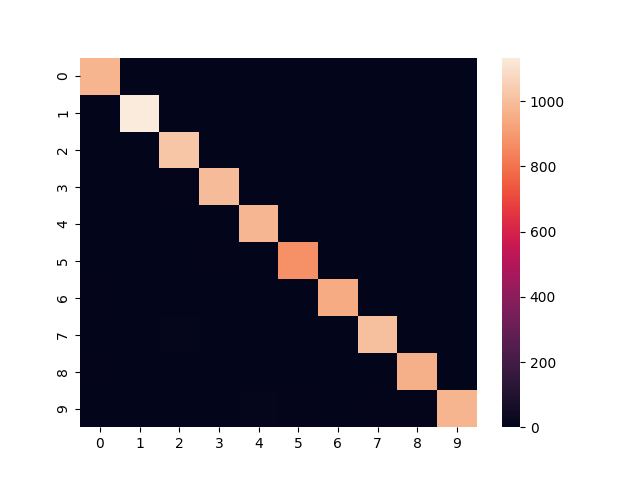
\includegraphics[width=0.55\textwidth]{author/part3/figures/conf_matrix_result.png}
	\caption{Матрица ошибок для задачи MNIST}
	\label{fig:conf_matrix_result}
\end{figure}

Мы получили матрицу с явно выраженным диагональным преобладанием, таким образом полученная модель делает относительно небольшое число ошибок.

Исходя из анализа этапов построения и.н.с., которые выполняют разработчики, можно вывести следующую классификацию действий по построению и.н.с.:

\begin{SCn}
	\scnheader{действие по построению и.н.с.}
	\begin{scnrelfromset}{декомпозиция}
		\scnitem{действие по обработке выборки}
		\begin{scnrelfromset}{декомпозиция}
			\scnitem{действие поиска подходящей обучающей выборки}
			\scnitem{действие формирования требований к обучающей выборке}
			\scnitem{действие очистки выборки}
			\scnitem{действие выявления содержательных признаков}
			\scnitem{действие трансформации выборки}
			\scnitem{действие разбиения выборки}
		\end{scnrelfromset}

		\scnitem{действие по проектированию и.н.с.}
		\begin{scnrelfromset}{декомпозиция}
			\scnitem{действие выбора класса нейросетевых методов}
			\scnitem{действие формирования спецификации входов и выходов и.н.с.}
		\end{scnrelfromset}

		\scnitem{действие обучения и.н.с.}
		\begin{scnrelfromset}{декомпозиция}
			\scnitem{действие выбора метода оптимизации}
			\scnitem{действие выбора минимизируемой функции ошибки}
			\scnitem{действие начальной инициализации и.н.с.}
			\scnitem{действие выбора гиперпараметров и.н.с.}
			\scnitem{действие обучения и.н.с.}
			\scnitem{действие оценки эффективности и.н.с.}
		\end{scnrelfromset}
	\end{scnrelfromset}
\end{SCn}

Реализация интерпретатора описанных в данной главе действий по построению и.н.с. и описания в базе знаний экспертных знаний разработчиков и.н.с. (а значит реализация интеллектуальной среды проектирования и.н.с.) позволит автоматически, исходя из описания задачи, генерировать нейросетевые методы в памяти ostis-системы, что является одним из ключевых направлений развития данной работы.

Так как в результате действий по построению и.н.с. объект этих действий, конкретная и.н.с., может существенно меняться (меняется конфигурация сети, ее весовые коэффициенты), то и.н.с. представляется в базе знаний как темпоральное объединение всех ее версий. Каждая версия является  \textit{и.н.с.} и темпоральной сущностью. На множестве этих темпоральных сущностей задается темпоральная последовательность с указанием первой и последней версии. Для каждой версии описываются специфичные знания.

Общие для всех версий знания описываются для и.н.с, являющейся темпоральным объединением всех версий (рисунок \nameref{fig:temporal_neural_network_scg})

\begin{figure}[H]
	\centering
	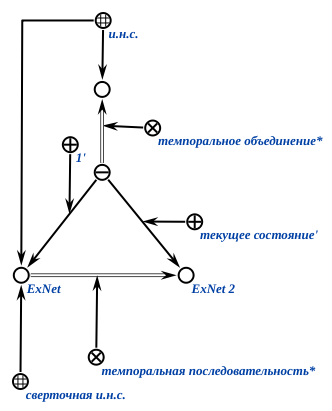
\includegraphics[scale=0.8]{author/part3/figures/temporal_neural_network_scg.png}
	\caption{Темпоральность нейронной сети}
	\label{fig:temporal_neural_network_scg}
\end{figure}

Далее более подробно рассмотрим действие по обучению \textit{и.н.с.} и сделаем обзор основных методов, применяемых для обучения.

\section*{Заключение к Главе \ref{chapter_ann}}
В главе описан подход к интеграции и конвергенции искусственных нейронных сетей с базами знаний в интеллектуальных компьютерных системах нового поколения с помощью представления и интерпретации искусственной нейронной сети в базе знаний.

Описаны синтаксис, денотационная и операционная семантика языка представления нейросетевых методов, который позволяет представить и интерпретировать в памяти интеллектуальной системы любую и.н.с. Наличие такого языка порождает семантическую совместимость нейросетевого метода с другими методами, представленными в памяти системы, что позволяет анализировать саму и.н.с. и этапы ее работы любыми другими методами системы.

Так же наличие языка представления нейросетевых методов позволяет описывать в памяти системы экспертные знания разработчиков и.н.с. В работе приведены этапы построения и.н.с., которые выполняют разработчики и.н.с. На основании этих этапов, c целью проектирования интеллектуальной среды построения нейросетевых методов, в базе знаний были классифицированы и описаны действия по построению и.н.с.

Проектирования и реализация интеллектуальной среды построения и.н.с. в базе знаний системы является одним из двух основных направлений дальнейшего развития данной работы.

Вторым основным направлением является разработка подхода к обработке фрагментов базы знаний с помощью и.н.с., для чего необходимо разработать универсальный алгоритм взаимно-однозначного соответствия фрагментов базы знаний и входных векторов и.н.с. Язык представления знаний способен представить любое знание. Наличие в системе нейросетевого метода, способного принимать на вход фрагменты знаний, позволит решить новые, слабо изученные классы задач. 